 \chapter{Resultados e Discussões}\label{cap:resultados}

Este estudo conta com a realização de testes nas bases de dados da UCI Machine Learning\footnote{http://archive.ics.uci.edu/ml/} - um repositório de dados a serviço da comunidade de aprendizado de máquina, criado por estudantes de pós-graduação na UC Irvine em 1987, e são bases utilizadas por educadores e pesquisadores como fonte primária de aplicações de aprendizado de máquina. 

%* lembrar que as bases são essas (iris, ...) por serem já estudadas, e de prévio conhecimento, onde a partir de estudos em bases assim pode-se ter resultados conclusivos e expandir para outras bases. É como se testase com base conhecida para depois pegar uma nova.

As bases de dados escolhidas para este trabalho foram: Seeds, Iris, Glass, Wine. Essas bases são bastantes utilizadas em vários trabalhos\footnote{https://archive.ics.uci.edu/ml/datasets/glass+identificpation, https://archive.ics.uci.edu/ml/datasets/iris, https://archive.ics.uci.edu/ml/datasets/wine, https://archive.ics.uci.edu/ml/datasets/seeds}, e através deles há possilidade de análises de seus comportamentos mediante seus resultados, visto que, todas as bases são classificadas, e já possuem seus grupos definidos, servindo de referência para  comparar  os resultados desta pesquisa. Sem esquecer que será trabalhado com os \textit{clusters} já formados e não na formação dos mesmos. Outro motivo desta seleção das bases  é mitigar ao máximo a utilização das técnicas de \textit{Feature Engineering} \cite{Casari2018}, que são técnicas de manipulação de dados empregados na base para aplicação do algoritmo de aprendizado de máquina utilizados na fase de preparação dos dados.
 

As tabelas apresentadas como resposta dos algoritmos de rotulação para cada base de dados possuem o seguinte formato: a primeira coluna (\textbf{Cluster}) é um número que representa cada \textit{cluster} de forma sequencial, a segunda coluna (\textbf{Rótulos}) representado pelo par, \textbf{Atributo} e \textbf{Faixa}, o quais definem o rótulo do \textit{cluster} respectivo, podendo haver ou não mais atributos para compor o rótulo. A coluna \textbf{Relevância} tem a importância de informar o quanto, em porcentagem, aquele atributo é relacionado aos demais, na definição do rótulo daquele \textit{cluster}. A quinta coluna, \textbf{Fora da Faixa}, exibe o erro em quantidade de elementos que não estão naquela faixa definida naquele rótulo, e por último a \textbf{Acurácia Parcial}, o qual exibe, em porcentagem, o valor de acertos dos elementos que são representados pelo atributo e faixa da respectiva linha. 

A obtenção da acurácia dos \textit{clusters} só é possível porquê as bases de dados já possuem seus grupos definidos, por conseguinte, há o conhecimento de quais elementos fazem parte de um determinado grupo. Dessa maneira, qualquer resultado da aplicação dos algoritmos nos \textit{clusters} podem ser confrontadas com as informações dos \textit{clusters} inicialmente retirados da UCI Machine Learning, e assim, poderá ser calculado a porcentagem de acertos.

A divisão deste capítulo iniciará por uma explanação da implementação do trabalho explicando as ferramentas  utilizadas no desenvolvimento com configurações  de algumas variáveis, e cada seção referirá a uma base de dados utilizada, sendo esta, dividida em subseções para os seguintes algoritmos: Naive Bayes, CART e KNN.

\section{Implementação}\label{cap:resultados:sec:implement}

Para  gerar os resultados aqui escritos foram realizadas implementações utilizando a ferramenta MATLAB\footnote{http://www.mathworks.com/products/matlab/ ; versão: R2016a(9.0.0.341360); 64-bit (glnxa64)}, sendo possível utilizar suas funções de aprendizado de máquina já implementadas na \textit{Statistics and Machine Learning Toolbox }. Por aprensentar  linguagem técnica e funcões já prontas direcionada para aprendizado de máquina essa ferramenta foi selecionada para colocar em prática essa pesquisa.

Ao longo da pesquisa foram realizados vários testes, porém, houveram alterações de algumas variáveis e métodos de discretização, sempre com o objetivo de obter os melhores resultados. As variáveis e métodos alterados são: variância (${V}$), número de faixas (${R}$), e tipo de discretização, ${TipoDiscretização}$ (EWD,EFD). 

Fazendo um breve resumo sobre as configurações das variáveis, a variação ${V}$ existe para evitar a ambiguidade dos rótulos, ou seja, quando os rótulos apresentarem os mesmos resultados: atributo e faixa de valor. O número de faixas (${R}$), é o número de faixas definido de forma que os atributos tenham seus valores mapeados de acordo com o valor da variável, e dependendo de como os dados do atributo são dispostos, existirá uma melhor divisão no número de faixas \footnote{Explicação sobre o número de faixas no Apêndice \ref{apendice:1}}. Uma vez definido o número de faixas será escolhido qual método de discretização será aplicado (EWD,EFD), decidindo qual faixa cada valor irá ficar.  

%Além de evitar a ambiguidade dos rótulos a variável ${V}$ pode ser utilizada também para selecionar mais de um atributo para ser o rótulo do cluster. 


%A utilização da variação ${V}$ para escolha de rótulos acontece após uma análise da tabela de correlação dos atributos (seção \ref{cap:ferramentas:sec:tecnica}), a exemplo da tabela \ref{tab:matrelevancia:seeds:nb}. E existindo valores muito próximos em relação a outros (cabe a uma análise se necessário), poderá utilizar esses atributos também como rótulos para melhor definir o cluster. A variável ${V}$ pode ser configurada com um valor que possa abranger esses atributos que possuam valores de porcentagens próximos ao do atributo de maior valor na tabela (mais relevante). O valor de ${V}$ é subjetivo e sua adição é condicionada a análise da aplicação do algoritmo na bases de dados.

%É importante ressaltar a criação da tabela de correlação de atributos (Matriz de Atributos Importantes). Essa tabela é implementada conforme a técnica de correlação entre atributos com algoritmos supervisionados, seção \ref{cap:ferramentas:ssec:algsuper}, onde cada célula da tabela é preenchida através da execução de um algoritmo supervisionado. Estas execuções são realizadas em todos os atributos da cada cluster existente na base de dados.

%Após a tabela preenchida, o atributo rótulo será selecionado a partir do maior valor em relação aos outros atributos do grupo, que é representado pela linha da tabela (matriz de atributos). Também poderá ser selecionado como rótulo os atributos que possuam o valor entre a diferença de ${V}$ com o atributo de maior valor (mais relevante). Por exemplo, se o valor de ${V=5\%}$ e o atributo de maior valor é \textbf{95\%}, então todos os atributos que possuírem o valor a partir de \textbf{90\%} serão considerados rótulos também.

%a cada iteração do algoritmo é preenchida uma célula da tabela com o valor de correlação do primeiro atributo até o último atributo de um cluster, e depois iniciado o mesmo procedimento a outro cluster até não haver mais clusters. Após a tabela estar montada o atributo rótulo será selecionado a partir do maior valor em relação aos outros atributos do grupo, e caso seja necessário também é selecionado como rótulo os atributos que possuam o valor entre a diferença de ${V}$ com o atributo de maior valor (mais relevante). 


%A cada base de dados descritas nas seções seguintes, são configuradas algumas variáveis, método de discretização e implementado dois algoritmos de aprendizado supervisionado com paradigmas diferentes para fazer rotulação. Cada algoritmo terá como resultado o rótulo por cluster de dados.


\section{Base de Dados 1 - Seeds - Identificação de Tipos de Semente}
Essa base é composta por sete  atributos definindo suas características, e mais um atributo, classe,  responsável por identificar os tipos de sementes \cite{Charytanowicz2010}. Esses elementos foram construídos a partir de sete parâmetros geométricos medidos dos grãos de trigo: \textit{area} - A, \textit{perimeter} - P, \textit{compactness} - C, \textit{length of kernel} - Lkernel, \textit{width of kernel} - Wkernel, \textit{asymmetry coefficient} - asymetry, \textit{length of kernel groove} - lkgroove.

Os valores dos atributos  são todos contínuos e não existem valores em branco,  possuindo um total de 210 registros classificados em três categorias bem distribuidas entre as classes, definindo esta, como base de dados balanceada, por conta dessa distribuição dos registros:
\begin{itemize}[noitemsep]
 \item 70 elementos do tipo \textit{Kama};
 \item 70 elementos do tipo \textit{Rosa};
 \item 70 elementos do tipo \textit{Canadian}.
\end{itemize}
Para classificar as sementes, como \textit{Kama}, \textit{Rosa} e \textit{Canadian} foi utilizada uma técnica de raio X, que é relativamente mais barata que outras técnicas de imagem, como microscopia ou tecnologia a laser. O material foi colhido de campos experimentais, explorados no Instituto de Agrofísica da Academia Polonesa de Ciências em Lublin.


As tabelas com os resultados dos rótulos apresentadas a seguir (tabelas \ref{tab:rot:seeds:nb}, \ref{tab:rot:seeds:cart}, \ref{tab:rot:seeds:knn}) exibem os resultados de rotulação dos algoritmos Naive Bayes, CART e KNN, respectivamente, e no caso dos \textit{clusters}, cada linha determina um grupo: (1) \textit{Kama}, (2) \textit{Rosa} e (3) \textit{Canadian}. 


Como já mencionado neste capítulo, na seção \ref{cap:resultados:sec:implement}, antes de executar o algoritmo algumas configuração são necessárias para executar o algoritmo, como, a configuração do método de discretização que do tipo EFD, e também a divisão dos valores dos atributos em faixas, com ${R=3}$ para todos os atributos, e variação ${V=0\%}$ 

%e também o valor de variação ${V=0\%}$,  não obstante, esta variável ${V}$ só assumirar valor maior que zero após análise dos resultados caso haja ambiguidade.


\subsection{Naive Bayes} \label{cap:resultados:ssec:seed:nb}
% Please add the following required packages to your document preamble:
% \usepackage{multirow}
% \usepackage[table,xcdraw]{xcolor}
% If you use beamer only pass "xcolor=table" option, i.e. \documentclss[xcolor=table]{beamer}

%Para ter maior clareza na escolha desses atributos foi inseridaa a tabela \ref{tab:matrelevancia:seeds:nb} que exibem os valores de correlação entre eles.


Na tabela \ref{tab:rot:seeds:nb} pode-se verificar o resultado da aplicação do algoritmo, e através dela percebe-se que em 2 (dois) clusters obtiveram acurácia acima de 90\% (noventa porcento), indicando um rótulo que representa bem o \textit{cluster}. A partir das colunas  \textbf{Fora da Faixa} e Acurácia Parcial, pode-se ter um indicativo bom ou ruim do rótulo nos clusters, e  logo na linha representada pelo \textit{cluster} 1 (um), é exibido 14 (quatorze) elementos que não estão participando da faixa definida pelo rótulo, isso implica que aquele rótulo não consegue representar esses 14 (quatorze) elementos que fazem parte do \textit{cluster} 1 (um). Já na segunda linha que representa o segundo \textit{cluster} houve um erro de 6 (seis) elementos que não foram representados pelo rótulo, e o rótulo que mais representou o grupo foi o do \textit{cluster} 3 (três) o qual obteve um atributo com relevância de 95\% (noventa e cinco) entre os demais atributos, e com menor números de elementos fora da faixa totalizando os 5 (cinco) elementos. %entre os 70 (setenta) do \textit{cluster} 3.


\begin{table}[!h]
\centering
\caption{Resultado da rotulação com o algoritmo Naive Bayes}
\label{tab:rot:seeds:nb}
\scalebox{0.8}{
\begin{tabular}{llcrcc}
\hline \hline
\multicolumn{1}{c}{\cellcolor[HTML]{FFFFFF}} & \multicolumn{2}{c}{Rótulos}                & \multicolumn{1}{r}{}               & & \\ \cline{2-3}
Cluster                                      & Atributos      & \multicolumn{1}{c}{Faixa} & \multicolumn{1}{c}{Relevância(\%)} & Fora da Faixa & Acurácia Parcial(\%) \\ \hline \hline
1                                            & area           & ] 12.78 $\sim$  16.14 ]   & 92\%                               & 14 & 80\% \\  \hline
2                                            & area           & ] 16.14 $\sim$  21.18 ]   & 95\%                               & 6 & 91,4\%\\ \hline
%\multirow{-2}{*}{2}                          & lkernel        & ] 5.826 $\sim$  6.675 ]   & 92\%                               & 6\\  \hline
3                                            & perimetro      & [ 12.41 $\sim$  13.73 ]   & 95\%                               & 5 & 92,8\% \\ \hline \hline
\end{tabular}
}
\end{table}




Na última coluna, \textbf{Acurácia Parcial}, apresenta em porcentagem o grau de acerto, por \textit{cluster}, dos registros que são representados pelo rótulo. Essa acurácia é possível, visto que, na descrição do \textit{dataset} da  \textit{UCI Machine Learning}\footnote{repositório de dados de onde está a base de dados. https://archive.ics.uci.edu/ml/datasets/seed} já é definido que cada grupo possui 70 (setenta) registros, e quais elementos fazem parte de cada \textit{cluster}. Dessa forma o melhor rótulo ficou no \textit{cluster} 3 (três), \textit{Canadian}, que ficou com 92,8\% (noventa e dois vírgula oito porcento) de acurácia.

Analisando a coluna \textbf{Rótulos} da tabela \ref{tab:rot:seeds:nb}, nota-se que o atributo \textbf{area} aparece tanto no  \textit{cluster} 1 (um) como também no \textit{cluster} 2 (dois). A rotulação de dados envolve não só o atributo mais relevante, como também, a faixa de valores, onde é contado os elementos que mais se repetem dentro do atributo. Nesse caso, pode-se observar que na coluna \textbf{Atributos}, mesmo possuindo  \textbf{area} como parte do rótulo, nos \textit{cluster}  1 (um) e 2 (dois), as faixa de valores diferem uma da outra, sendo considerados rótulos distintos, todavia os rótulos seriam iguais, somente se, a tupla, atributo e faixa, fossem iguais.


%Caso os resultados gerados na tabela \ref{tab:matrelevancia:seeds:nb} expusessem clusters com rótulos ambíguos, poderia ser utilizado a variação de ${V}$. Quando houver ambiguidade dos rótulos, a seleção dos atributos que compõem os rótulos, acontecerá da diferença da variável ${V}$ em relação ao atributo de maior relevência do cluster. Caso essa variável tenha o valor alterado, os rótulos dos clusters poderão sofrer mudanças, pois poderia aumentar  ou diminuir o número de atributos dos rótulos, dependendo do valor inserido em ${V}$. Através da tabela \ref{tab:matrelevancia:seeds:nb} é possível analisar todos os valores de relevância gerados para os atributos e analisar qual valor pode-se inserir em ${V}$ para montar o rótulo.

%Para exemplificar a utilização da variável ${V}$ pode-se utilizar como exemplo os dados do cluster 2 da tabela \ref{tab:matrelevancia:seeds:nb} e adotando ${V=3\%}$.  Neste exemplo não só o atributo de maior relevância, \textbf{area} com ${95.7\%}$ seria escolhido como rótulo, mas também o atributo \textbf{lkernel} com valor ${92.8\%}$, pois a diferença entre o valor de \textbf{area} com ${V}$ resultaria em ${92.7\%}$. Através dessa diferença todos os atributos que estivessem na faixa de ${92.7\%}$ a  ${95.7\%}$ seriam selecionados como atributos do rótulo.
% 
% \begin{table}[!h]
%     
%     \caption{Resultado da Correlação dos atributos pelo Naive Bayes; Legenda dos Atributos: (A)area, (B)perimetro, (C)compacteness, (D)Lkernel, (E)Wkernel, (F)asymetry, (G)lkgroove}    
%     \centering
%    \small\addtolength{\tabcolsep}{+2pt}
%     \begin{tabular}{|cl|c|c|c|c|c|c|c|}
%         \hline \hline
%                                 &   & \multicolumn{7}{c|}{Atributos}          \\ \cline{3-9} 
%         \multicolumn{1}{|l}{}                            &   & A    & B & C & D & E & F & G \\ \hline
%         \multicolumn{1}{|c|}{}                           & 1 & 92.8 & 87.1   & 50.0      & 75.7 & 85.7 & 60.0   & 65.7   \\ \cline{2-9} 
%         \multicolumn{1}{|c|}{}                           & 2 & 95.7 & 91.4   & 47.1      & 92.8 & 90.0 & 28.5  & 85.7  \\ \cline{2-9} 
%         \multicolumn{1}{|c|}{\multirow{-3}{*}{Clusters}} & 3 & 91.4 & 95.7   & 71.4      & 85.7 & 91.4 & 64.2  & 58.5  \\ \hline
%     \end{tabular}
%     \label{tab:matrelevancia:seeds:nb} 
% \end{table}

%A tabela \ref{tab:matrelevancia:seeds:nb} é um exemplo da matriz de atributos importantes gerada pela técnica de correlação entre atributos. É formada por clusters representado pelas linhas, e atributos representado por colunas, onde esses valores são representados em porcentagem (\%). 

%Essa tabela é fruto da aplicação do Naive Bayes na base de dados \textbf{Seeds}, e a partir dela é retirado o(s) atributo(s) rótulo(s). Uma análise pode ser feita através desses dados e ajudar a definir um valor para a variável ${V}$ caso necessário. Percebe-se que algumas características são mais bem correlacionadas que  outras, através dos valores mais altos indicando o grau de relacionamento entre os atributos após a aplicação do algoritmo. 

% 
% \begin{table}[!h]
% \caption{Resultado de 4 (quatro) execuções do algoritmo Naive Bayes; Legenda dos Atributos: (A)area, (B)perimetro, (C)compacteness, (D)Lkernel, (E)Wkernel, (F)asymetry, (G)lkgroove}
%  %\begin{tabular}{ll}
% %\rule{0}{50}
% \centering
%    \subfloat[1a. Execução]{ \label{tab:execucoes:seed:nb:1exec}
%    %\scalebox{0.5}{%
%    \small\addtolength{\tabcolsep}{-2pt} 
%      \begin{tabular}{|cl|c|c|c|c|c|c|c|}
%         \hline \hline
%             {\tiny 1a. Execução}     &   & \multicolumn{7}{c|}{Atributos}                                               \\ \cline{3-9} 
%        \multicolumn{1}{|l}{}                            &   & A    & B & C & D & E & F & G \\ \hline
%         \multicolumn{1}{|c|}{}                           & 1 & 92.8 & 87.1   & 48.5      & 77.1 & 82.8 & 57.1   & 65.7   \\ \cline{2-9} 
%         \multicolumn{1}{|c|}{}                           & 2 & 94.2 & 90.0   & 45.7      & 92.8 & 90.0 & 38.5  & 87.1  \\ \cline{2-9} 
%         \multicolumn{1}{|c|}{\multirow{-3}{*}{Clusters}} & 3 & 91.4 & 95.7   & 72.8      & 85.7 & 91.4 & 64.2  & 60.0  \\ \hline
%       \end{tabular}
%     %}
%     }
%  %&
%  %\hspace{1cm} %altera o espaçamento entre as tabelas
%  
%    \subfloat[2a. Execução]{ \label{tab:execucoes:seed:nb:2exec}
%  %\scalebox{0.5}{%
%    \small\addtolength{\tabcolsep}{-2pt}
%    \begin{tabular}{|cl|c|c|c|c|c|c|c|}
%         \hline \hline
%              {\tiny 2a. Execução }       &   & \multicolumn{7}{c|}{Atributos}                                               \\ \cline{3-9} 
%        \multicolumn{1}{|l}{}                            &   & A    & B & C & D & E & F & G \\ \hline
%         \multicolumn{1}{|c|}{}                           & 1 & 92.8 & 87.1   & 47.1      & 77.1 & 87.1 & 60.0   & 65.7   \\ \cline{2-9} 
%         \multicolumn{1}{|c|}{}                           & 2 & 94.2 & 90.0   & 47.1      & 92.8 & 91.4 & 32.8  & 87.1  \\ \cline{2-9} 
%         \multicolumn{1}{|c|}{\multirow{-3}{*}{Clusters}} & 3 & 91.4 & 95.7   & 72.8      & 85.7 & 92.8 & 64.2  & 60.0  \\ \hline
%       \end{tabular}
%   %}
%   %\\  [8ex]
%     }
%     
%     \subfloat[3a. Execução]{ \label{tab:execucoes:seed:nb:3exec}
%  %\scalebox{0.5}{%
%    \small\addtolength{\tabcolsep}{-2pt} 
%    \begin{tabular}{|cl|c|c|c|c|c|c|c|}
%         \hline \hline
%           {\tiny 3a. Execução}     &   & \multicolumn{7}{c|}{Atributos}                                               \\ \cline{3-9} 
%        \multicolumn{1}{|l}{}                            &   & A    & B & C & D & E & F & G \\ \hline
%         \multicolumn{1}{|c|}{}                           & 1 & 94.2 & 85.7   & 48.5      & 77.1 & 82.8 & 61.4   & 65.7   \\ \cline{2-9} 
%         \multicolumn{1}{|c|}{}                           & 2 & 92.8 & 90.0   & 50.0      & 92.8 & 90.0 & 32.8  & 87.1  \\ \cline{2-9} 
%         \multicolumn{1}{|c|}{\multirow{-3}{*}{Clusters}} & 3 & 91.4 & 95.7   & 72.8      & 85.7 & 92.8 & 64.2  & 60.0  \\ \hline
%    \end{tabular}
%     }
%     %&
%     
%     \subfloat[4a. Execução]{  \label{tab:execucoes:seed:nb:4exec}
%        \small\addtolength{\tabcolsep}{-2pt}
%         \begin{tabular}{|cl|c|c|c|c|c|c|c|}
%         \hline \hline
%             {\tiny 4a. Execução }   &   & \multicolumn{7}{c|}{Atributos}                                               \\ \cline{3-9} 
%        \multicolumn{1}{|l}{}                            &   & A    & B & C & D & E & F & G \\ \hline
%         \multicolumn{1}{|c|}{}                           & 1 & 91.4 & 88.5   & 54.2      & 75.7 & 85.7 & 62.8   & 61.4   \\ \cline{2-9} 
%         \multicolumn{1}{|c|}{}                           & 2 & 95.7 & 90.0   & 50.0      & 92.8 & 90.0 & 38.5  & 85.7  \\ \cline{2-9} 
%         \multicolumn{1}{|c|}{\multirow{-3}{*}{Clusters}} & 3 & 91.4 & 95.7   & 72.8      & 85.7 & 94.2 & 64.2  & 57.1  \\ \hline
%         \end{tabular}
%    %\\
%     }
%     
%  %\end{tabular}
%  \label{tab:execucoes:seed:nb}
% \end{table}

%% TESTE DE CRIAÇÃO DE TABELA
% \begin{table}[!h]
% \caption{Resultado de 4 (quatro) execuções do algoritmo Naive Bayes; Legenda dos Atributos: (A)area, (B)perimetro, (C)compacteness, (D)Lkernel, (E)Wkernel, (F)asymetry, (G)lkgroove}
%  \centering
%  \subfloat[Tabela A]{
%  
%  \small\addtolength{\tabcolsep}{-5pt}
%  \begin{tabular}{|cl|c|c|c|c|c|c|c|}
%         \hline \hline
%             {\tiny 1a. Execução}     &   & \multicolumn{7}{c|}{Atributos}                                               \\ \cline{3-9} 
%        \multicolumn{1}{|l}{}                            &   & A    & B & C & D & E & F & G \\ \hline
%         \multicolumn{1}{|c|}{}                           & 1 & 92.8 & 87.1   & 48.5      & 77.1 & 82.8 & 57.1   & 65.7   \\ \cline{2-9} 
%         \multicolumn{1}{|c|}{}                           & 2 & 94.2 & 90.0   & 45.7      & 92.8 & 90.0 & 38.5  & 87.1  \\ \cline{2-9} 
%         \multicolumn{1}{|c|}{\multirow{-3}{*}{Clusters}} & 3 & 91.4 & 95.7   & 72.8      & 85.7 & 91.4 & 64.2  & 60.0  \\ \hline
%       \end{tabular}
%  }
%  
%  %\hspace{3cm}
%  
%  \subfloat[Tabela B]{
%  
%  \small\addtolength{\tabcolsep}{-5pt}
%  \begin{tabular}{|cl|c|c|c|c|c|c|c|}
%         \hline \hline
%             {\tiny 1a. Execução}     &   & \multicolumn{7}{c|}{Atributos}                                               \\ \cline{3-9} 
%        \multicolumn{1}{|l}{}                            &   & A    & B & C & D & E & F & G \\ \hline
%         \multicolumn{1}{|c|}{}                           & 1 & 92.8 & 87.1   & 48.5      & 77.1 & 82.8 & 57.1   & 65.7   \\ \cline{2-9} 
%         \multicolumn{1}{|c|}{}                           & 2 & 94.2 & 90.0   & 45.7      & 92.8 & 90.0 & 38.5  & 87.1  \\ \cline{2-9} 
%         \multicolumn{1}{|c|}{\multirow{-3}{*}{Clusters}} & 3 & 91.4 & 95.7   & 72.8      & 85.7 & 91.4 & 64.2  & 60.0  \\ \hline
%       \end{tabular}
%  }
%  
% \end{table}



%Para provar empiricamente os resultados, na tabela \ref{tab:execucoes:seed:nb} é exposto  4 (quatro) execuções do Algoritmo Naive Bayes. Pode-se constatar que mesmo havendo algumas alterações nos valores dos atributos em cada execução, a correlação entre os atributos não oferece muita alteração. Como exemplo, o atributo \textbf{area} nos clusters 1 e 2, possuem o melhor grau de correlacionamento em seus grupos, mesmo nas quatro execuções, como mostrado na tabela \ref{tab:execucoes:seed:nb}.

%A informação passada pela tabela \ref{tab:execucoes:seed:nb} tem a intenção de mostrar para o analista que estiver aplicando a rotulação de dados, como seus atributos se comportam em cada cluster, ao utilizar  o método de rotulação de dados.

Segue abaixo o resultado do algoritmo Naive Bayes na base de dados \textbf{Seeds} com seus rótulos: 
\begin{itemize}[noitemsep]
 \item ${r_{c_1}=\{ (area, ]12.78 \sim 16.14]) \} }$  
 \item ${r_{c_2}=\{ (area, ]16.14 \sim 21.18]) \} }$
 \item ${r_{c_3}=\{ (perimetro, [12.41 \sim 13.73])\} }$
\end{itemize}


\subsection{Classification and Regression Trees - CART}\label{cap:resultados:ssec:seed:cart}

Na tabela \ref{tab:rot:seeds:cart}, que segue o mesmo modelo anterior, tem-se o resultado da aplicação do algoritmo supervisionado na base Seeds. O CART é utilizado pela toolbox do MATLAB como algoritmo de classificação de árvore de decisão. 
%O que se pretende fazer é seguir a pesquisa e testar a base de dados com um paradigma  diferente para fazer rotulação nos clusters.

\begin{table}[!h]
\centering
\caption{Resultado da aplicação do algoritmo CART}
\label{tab:rot:seeds:cart}
\scalebox{0.8}{
\begin{tabular}{llcrcc}\hline \hline

\multicolumn{1}{c}{\cellcolor[HTML]{FFFFFF}} & \multicolumn{2}{c}{Rótulos}                      & \multicolumn{1}{r}{}            \\ \cline{2-3}
Parcial                                      & Atributos      & \multicolumn{1}{c}{Faixa}       & \multicolumn{1}{c}{Relevância(\%)} & Fora da Faixa & Acurácia Cluster(\%)\\ \hline \hline
%                                             & area           & ] 12.78 $\sim$  16.14 ]         & 91\%          & 14 \\  
1                                            & perimetro      & [ 13.73 $\sim$ 15.18 ]          & 94\%          & 14 & 80\%\\ \hline
                                             & area           & ] 16.14 $\sim$  21.18 ]          & 98\%         & 6 & 91\%\\ 
\multirow{-2}{*}{2}                          & perimetro      & ] 15.18 $\sim$  17.25 ]          & 98\%         & 7 & 90\% \\  \hline
%                                             & perimetro      & [ 12.41 $\sim$  13.73 ]         & 95\%          & 5 \\
3                                            & wkernel        & [ 2.63 $\sim$  3.049 ]         & 97\%           & 9 & 87,1\%\\ \hline \hline
\end{tabular}}
\end{table}

O resultado desse algoritmo,  teve escolhas dos atributos de cada rótulo dos \textit{clusters}  diferentes ao do Naive Bayes visto anteriormente, e a coluna \textbf{Fora da Faixa} teve valores um pouco maiores em alguns \textit{clusters}, que por consequência houve uma acurácia menor entre os \textit{clusters}. 

Logo, na tabela \ref{tab:execucoes:seed:cart} é exibida a matriz de atributos importantes, a qual possui os valores de correlação entre os demais atributos, como também os valores de correlação dos atributos rótulos, destacados. Essas informações ajudam a entender como o atributo rótolo é escolhido, podendo ser um ou mais atributos. 
\begin{table}[!h]
\centering
\caption{Matriz de Atributos Importantes do algoritmo CART na base Seeds}
\label{tab:execucoes:seed:cart}
\scalebox{0.8}{
\begin{tabular}{|cl|c|c|c|c|c|c|c|}
        \hline \hline
           {\tiny  }      &   & \multicolumn{7}{c|}{Atributos}                                               \\ \cline{3-9} 
       \multicolumn{1}{|l}{}                            &   & area    & perimetro & compacteness & Lkernel & Wkernel & asymetry & lkgroove \\ \hline
        \multicolumn{1}{|c|}{}                           & 1 & 91.4 & \textbf{94.2}   & 58.5      & 80.0 & 74.2 & 55.7   & 60.0   \\ \cline{2-9} 
        \multicolumn{1}{|c|}{}                           & 2 & \textbf{98.5} & \textbf{98.5}   & 50.0      & 90.0 & 88.5 & 41.4  & 90.0  \\ \cline{2-9} 
        \multicolumn{1}{|c|}{\multirow{-3}{*}{Clusters}} & 3 & 92.8 & 95.7   & 80.0      & 88.5 & \textbf{97.1} & 55.7  & 77.1  \\ \hline
      \end{tabular}}
\end{table}   

No \textit{cluster} 2 (dois) houve um empate no valor de relevância de dois atributos, implicando na escolha de ambos para integrar o rótulo. Isso acontece quando na execução do algoritmo, na etapa da escolha do maior valor do atributo para ser rótulo na matriz de atributos importantes (tabela \ref{tab:execucoes:seed:cart}), há no mesmo \textit{cluster}, valores de atributos iguais, não importando a quantidade de atributos com valores ambíguos. 
 
    
%Já na tabela \ref{tab:execucoes:seed:cart} são exibidas algumas execuções do algoritmo CART na base de dados. O mesmo comportamento entre execuções pode ser visto no algoritmo de paradigma estatístico, subseção \ref{cap:resultados:ssec:seed:nb}, realizado nessa pesquisa. O  comportamento de ambos os algoritmos foram bem semelhantes, como também, seus valores nas execuções que não se alteraram muito a cada iteração.
%%%%%%%%%%%%%%%%%%%%%%%%%%%%%%%%%%%%%%%%%%%%%%%%%%%%%%%%
% 
% \begin{table}[!h]
% \caption{Resultado de 4 (quatro) execuções do algoritmo Naive Bayes; Legenda dos Atributos: (A)area, (B)perimetro, (C)compacteness, (D)Lkernel, (E)Wkernel, (F)asymetry, (G)lkgroove}
%  %\begin{tabular}{ll}
% %\rule{0}{50}
% \centering
%    \subfloat[1a. Execução]{ \label{tab:execucoes:seed:cart:1exec}
%    %\scalebox{0.5}{%
%    \small\addtolength{\tabcolsep}{-2pt} 
%     \begin{tabular}{|cl|c|c|c|c|c|c|c|}
%         \hline \hline
%            {\tiny  1a. Execução}      &   & \multicolumn{7}{c|}{Atributos}                                               \\ \cline{3-9} 
%        \multicolumn{1}{|l}{}                            &   & A    & B & C & D & E & F & G \\ \hline
%         \multicolumn{1}{|c|}{}                           & 1 & 91.4 & 94.2   & 58.5      & 80.0 & 74.2 & 55.7   & 60.0   \\ \cline{2-9} 
%         \multicolumn{1}{|c|}{}                           & 2 & 98.5 & 98.5   & 50.0      & 90.0 & 88.5 & 41.4  & 90.0  \\ \cline{2-9} 
%         \multicolumn{1}{|c|}{\multirow{-3}{*}{Clusters}} & 3 & 92.8 & 95.7   & 80.0      & 88.5 & 97.1 & 55.7  & 77.1  \\ \hline
%       \end{tabular}
%     %}
%     }
%  %&
%  %\hspace{1cm} %altera o espaçamento entre as tabelas
%  
%    \subfloat[2a. Execução]{ \label{tab:execucoes:seed:cart:2exec}
%  %\scalebox{0.5}{%
%    \small\addtolength{\tabcolsep}{-2pt}
%   \begin{tabular}{|cl|c|c|c|c|c|c|c|}
%         \hline \hline
%          {\tiny  2a. Execução} &   & \multicolumn{7}{c|}{Atributos}                                               \\ \cline{3-9} 
%        \multicolumn{1}{|l}{}                            &   & A    & B & C & D & E & F & G \\ \hline
%         \multicolumn{1}{|c|}{}                           & 1 &  91.4 & 94.2   & 62.8      & 78.5 & 81.4 & 61.4   & 57.1   \\ \cline{2-9} 
%         \multicolumn{1}{|c|}{}                           & 2 & 98.5 & 98.5   & 54.2      & 90.0 & 88.5 & 40.0  & 90.0  \\ \cline{2-9} 
%         \multicolumn{1}{|c|}{\multirow{-3}{*}{Clusters}} & 3 & 92.8 & 95.7   & 80.0      & 88.5 & 97.1 & 60.0  & 77.1  \\ \hline
%       \end{tabular}
%   %}
%   %\\  [8ex]
%     }
%     
%     \subfloat[3a. Execução]{ \label{tab:execucoes:seed:cart:3exec}
%  %\scalebox{0.5}{%
%    \small\addtolength{\tabcolsep}{-2pt} 
%    \begin{tabular}{|cl|c|c|c|c|c|c|c|}
%         \hline \hline
%           {\tiny  3a. Execução}   &   & \multicolumn{7}{c|}{Atributos}                                               \\ \cline{3-9} 
%        \multicolumn{1}{|l}{}                            &   & A    & B & C & D & E & F & G \\ \hline
%         \multicolumn{1}{|c|}{}                           & 1 & 93.8 & 93.6   & 61.8      & 83.2 & 89.2 & 53.2   & 71.0   \\ \cline{2-9} 
%         \multicolumn{1}{|c|}{}                           & 2 & 98.2 & 98.3   & 61.9      & 93.0 & 90.5 & 25.2  & 90.1  \\ \cline{2-9} 
%         \multicolumn{1}{|c|}{\multirow{-3}{*}{Clusters}} & 3 & 95.5 & 96.3   & 82.4      & 90.9 & 97.7 & 59.3  & 77.0  \\ \hline
%    \end{tabular}
%     }
%     %&
%     
%     \subfloat[4a. Execução]{  \label{tab:execucoes:seed:cart:4exec}
%        \small\addtolength{\tabcolsep}{-2pt}
%    \begin{tabular}{|cl|c|c|c|c|c|c|c|}
%         \hline \hline
%          {\tiny 4a. Execução}       &   & \multicolumn{7}{c|}{Atributos}                                               \\ \cline{3-9} 
%        \multicolumn{1}{|l}{}                            &   & A    & B & C & D & E & F & G \\ \hline
%         \multicolumn{1}{|c|}{}                           & 1 & 92.8 & 94.2   & 60.0      & 80.0 & 84.2 & 64.2   & 60.0   \\ \cline{2-9} 
%         \multicolumn{1}{|c|}{}                           & 2 & 98.5 & 98.5   & 47.1      & 91.4 & 90.0 & 42.8  & 88.5  \\ \cline{2-9} 
%         \multicolumn{1}{|c|}{\multirow{-3}{*}{Clusters}} & 3 & 91.4 & 95.7   & 80.0      & 88.5 & 97.1 & 55.7  & 77.1  \\ \hline
%    \end{tabular}
%    %\\
%     }
%     
%  %\end{tabular}
%  \label{tab:execucoes:seed:cart}
% \end{table}
% %%%%%%%%%%%%%%%%%%%%%%%%%%%%%%%%%%%%%%%%%%%%%%%%%%%%%%%%%%%%%%%%%%%%

O resultado da rotulação utilizando o algoritmo CART na base de dados \textbf{Seeds} tem como rótulos: 
\begin{itemize}[noitemsep]
 \item ${r_{c_1}=\{ (perimetro, ]13.73 \sim 15.18]) \} }$
 \item ${r_{c_2}=\{ (area, ]16.14 \sim 21.18]), (perimetro, ]15.18 \sim 17.25]) \} }$
 \item ${r_{c_3}=\{ (wkernel, [2.63 \sim 3.049]) \} }$
\end{itemize}


\subsection{K-Nearest Neighbor - KNN} \label{cap:resultados:ssec:seed:knn}

Na tabela \ref{tab:rot:seeds:knn} aponta o \textit{cluster} 1 com o maior número de erros, diferente dos dois outros clusters, e diferente dos outros resultados o KNN apresenta no \textit{cluster} 3 um rótulo composto por dois atributos, que mesmo somado os erros, não ultrapassa os erros do \textit{cluster} 1.

\begin{table}[!h]
\centering
\caption{Resultado da aplicação do algoritmo KNN}
\label{tab:rot:seeds:knn}
\scalebox{0.8}{
\begin{tabular}{llcrcc}\hline \hline

\multicolumn{1}{c}{\cellcolor[HTML]{FFFFFF}} & \multicolumn{2}{c}{Rótulos}                      & \multicolumn{1}{r}{}            \\ \cline{2-3}
Parcial                                      & Atributos      & \multicolumn{1}{c}{Faixa}       & \multicolumn{1}{c}{Relevância(\%)} & Fora da Faixa & Acurácia Cluster(\%)\\ \hline \hline
%                                             & area           & ] 12.78 $\sim$  16.14 ]         & 91\%          & 14 \\  
1                                            & area      & ] 12.78 $\sim$ 16.14 ]          & 95\%          & 14 & 80\%\\ \hline
2                                            & Lkernel      & ] 5.83 $\sim$ 6.67 ]          & 94\%          & 6 & 91,4\%\\ \hline
                                             & area           & [ 10.59 $\sim$  12.78 ]          & 94\%         & 8 & 88\% \\ 
\multirow{-2}{*}{3}                          & perimetro        & [ 12.41 $\sim$  13.73 ]         & 94\%           & 5 & 92\% \\  \hline \hline

\end{tabular}}
\end{table}

O resultado da rotulação utilizando o algoritmo KNN na base de dados \textbf{Seeds} tem como rótulos: 
\begin{itemize}[noitemsep]
 \item ${r_{c_1}=\{ (area, ]12.78 \sim 16.14]) \} }$
 \item ${r_{c_2}=\{ (Lkernel, ]5.83 \sim 6.67]) \} }$
 \item ${r_{c_3}=\{ (area, [10.59 \sim 12.78]), (perimetro, [12.41 \sim 13.73]) \} }$
 
\end{itemize}


\subsection{Comparativo entre Algoritmos na Base de Dados Seeds} \label{cap:resultados:ssec:compalgoritmos:seeds}

Na aplicação do algoritmo KNN percebe-se coincidir o resultado somente no \textit{cluster} 1 com o Naive Bayes, não ocorrendo resultados semelhantes com o CART, e a acurácia nos três algoritmos foram a mesma. Considerando o rótulo do \textit{cluster} 2, os resultados ficaram diferentes, mas no KNN e Naive Bayes tiveram o mesmo poder de representatividade  deste \textit{cluster}, deixando de representar somente 6 (seis) elementos dos 70, do grupo \textit{Rosa} (\textit{cluster} 2), e no CART coincidiu um atributo do rótulo do Naive Bayes, mas apareceu outro atributo componto o rótulo. Já no \textit{cluster} 3 houve resultado parecido com o Naive Bayes, mas no KNN foi adicionado o  atributo \textbf{area} para compor o rótulo.


Para o melhor compreensão do rótulo do \textit{cluster} 1, desse e dos demais  algoritmos, será exibida a tabela \ref{tab:analise:seeds:cluster1}, representando os registros do grupo \textit{Kama}. Como os resultados de rotulação do KNN e Naive Bayes foram iguais no \textit{cluster} 1, a comparação será com os erros do KNN e CART (linhas destacadas), e a partir dessa tabela, pode-se acompanhar quais são os registros que são representados pelo rótulo e os que não são representados (Fora da Faixa). 


\begin{table}[!ht]
\caption{Parte dos dados pertencentes ao \textit{cluster} 1 (\textit{Kama}) - da base Seeds. No total são 210 registros os quais as linha de 1 a 70 são \textit{Kama}, 71 a 140 são Rosa e 141 a 210 são \textit{Canadian} }
 %\begin{tabular}{ll}
%\rule{0}{50}
\centering
   \subfloat[Amostra de dados ordenados em relação ao atributo \textbf{area}, representando os registros do grupo \textit{Kama} (\textit{cluster} 1)]{ \label{tab:analise:seeds:cluster1:bayes}
   %\scalebox{0.5}{%
   \small\addtolength{\tabcolsep}{-2pt} 
   \begin{tabular}{|c|c|c|c|c|c|c|c|}
\hline

& \textbf{area} & perimetro & compacteness & Lkernel & wkernel & asymetry &lkgroove \\ \hline
\rowcolor[HTML]{EFEFEF} 
1 & \textbf{11.23} & 12.63 & 0.884 & 4.902 & 2.879 & 2.269 & 4.703\\ \hline 
\rowcolor[HTML]{EFEFEF}
2 & \textbf{11.42} & 12.86 & 0.8683 & 5.008 & 2.85 & 2.7 & 4.607\\ \hline 
\rowcolor[HTML]{EFEFEF}
3 & \textbf{12.08} & 13.23 & 0.8664 & 5.099 & 2.936 & 1.415 & 4.961\\ \hline 
\rowcolor[HTML]{EFEFEF}
4 & \textbf{12.11} & 13.47 & 0.8392 & 5.159 & 3.032 & 1.502 & 4.519\\ \hline 
\rowcolor[HTML]{EFEFEF}
5 & \textbf{12.36} & 13.19 & 0.8923 & 5.076 & 3.042 & 3.22 & 4.605\\ \hline 
\rowcolor[HTML]{EFEFEF}
6 & \textbf{12.72} & 13.57 & 0.8686 & 5.226 & 3.049 & 4.102 & 4.914\\ \hline 
\rowcolor[HTML]{EFEFEF}
7 & \textbf{12.73} & 13.75 & 0.8458 & 5.412 & 2.882 & 3.533 & 5.067\\ \hline 
\rowcolor[HTML]{EFEFEF}
8 & \textbf{12.74} & 13.67 & 0.8564 & 5.395 & 2.956 & 2.504 & 4.869\\ \hline 
\rowcolor[HTML]{EFEFEF}
9 & \textbf{12.78} & 13.57 & 0.8716 & 5.262 & 3.026 & 1.176 & 4.782\\ \hline 
10 & \textbf{12.88} & 13.5 & 0.8879 & 5.139 & 3.119 & 2.352 & 4.607\\ \hline 
... & ... & ... & ... & ... & ... & ... & ...\\ \hline 
65 & \textbf{16.14} & 14.99 & 0.9034 & 5.658 & 3.562 & 1.355 & 5.175\\ \hline 
\rowcolor[HTML]{EFEFEF}
66 & \textbf{16.19} & 15.16 & 0.8849 & 5.833 & 3.421 & 0.903 & 5.307\\ \hline 
\rowcolor[HTML]{EFEFEF}
67 & \textbf{16.2} & 15.27 & 0.8734 & 5.826 & 3.464 & 2.823 & 5.527\\ \hline 
\rowcolor[HTML]{EFEFEF}
68 & \textbf{16.44} & 15.25 & 0.888 & 5.884 & 3.505 & 1.969 & 5.533\\ \hline 
\rowcolor[HTML]{EFEFEF}
69 & \textbf{16.63} & 15.46 & 0.8747 & 6.053 & 3.465 & 2.04 & 5.877\\ \hline 
\rowcolor[HTML]{EFEFEF}
70 & \textbf{17.08} & 15.38 & 0.9079 & 5.832 & 3.683 & 2.956 & 5.484\\ \hline  

\end{tabular}
    %}
    }
 %&
 %\hspace{1cm} %altera o espaçamento entre as tabelas
 \hspace{1cm}
   \subfloat[Amostra de dados ordenados em relação ao atributo \textbf{perimetro}  simulando os registros do \textit{cluster} 1]{ \label{tab:analise:seeds:cluster1:cart}
 %\scalebox{0.5}{%
   \small\addtolength{\tabcolsep}{-2pt}
   \begin{tabular}{|c|c|c|c|c|c|c|c|}
\hline

& area & \textbf{perimetro} & compacteness & Lkernel & wkernel & asymetry &lkgroove \\ \hline
\rowcolor[HTML]{EFEFEF} 
1 & 11.23 &\textbf{ 12.63} & 0.884 & 4.902 & 2.879 & 2.269 & 4.703\\ \hline 
\rowcolor[HTML]{EFEFEF} 
2 & 11.42 & \textbf{12.86} & 0.8683 & 5.008 & 2.85 & 2.7 & 4.607\\ \hline 
\rowcolor[HTML]{EFEFEF} 
3 & 12.36 & \textbf{13.19} & 0.8923 & 5.076 & 3.042 & 3.22 & 4.605\\ \hline 
\rowcolor[HTML]{EFEFEF} 
4 & 12.08 & \textbf{13.23} & 0.8664 & 5.099 & 2.936 & 1.415 & 4.961\\ \hline 
\rowcolor[HTML]{EFEFEF} 
5 & 12.11 & \textbf{13.47} & 0.8392 & 5.159 & 3.032 & 1.502 & 4.519\\ \hline 
\rowcolor[HTML]{EFEFEF} 
6 & 12.88 & \textbf{13.5} & 0.8879 & 5.139 & 3.119 & 2.352 & 4.607\\ \hline 
\rowcolor[HTML]{EFEFEF} 
7 & 13.16 & \textbf{13.55} & 0.9009 & 5.138 & 3.201 & 2.461 & 4.783\\ \hline 
\rowcolor[HTML]{EFEFEF} 
8 & 12.72 & \textbf{13.57} & 0.8686 & 5.226 & 3.049 & 4.102 & 4.914\\ \hline 
\rowcolor[HTML]{EFEFEF} 
9 & 12.78 & \textbf{13.57} & 0.8716 & 5.262 & 3.026 & 1.176 & 4.782\\ \hline 
\rowcolor[HTML]{EFEFEF} 
10 & 12.74 & \textbf{13.67} & 0.8564 & 5.395 & 2.956 & 2.504 & 4.869\\ \hline 
11 & 12.73 & \textbf{13.75} & 0.8458 & 5.412 & 2.882 & 3.533 & 5.067\\ \hline 
... & ... & ... & ... & ... & ... & ... & ...\\ \hline 
66 & 16.19 & \textbf{15.16} & 0.8849 & 5.833 & 3.421 & 0.903 & 5.307\\ \hline 
\rowcolor[HTML]{EFEFEF} 
67 & 16.44 & \textbf{15.25} & 0.888 & 5.884 & 3.505 & 1.969 & 5.533\\ \hline 
\rowcolor[HTML]{EFEFEF} 
68 & 16.2 & \textbf{15.27} & 0.8734 & 5.826 & 3.464 & 2.823 & 5.527\\ \hline 
\rowcolor[HTML]{EFEFEF} 
69 & 17.08 & \textbf{15.38} & 0.9079 & 5.832 & 3.683 & 2.956 & 5.484\\ \hline 
\rowcolor[HTML]{EFEFEF} 
70 & 16.63 & \textbf{15.46} & 0.8747 & 6.053 & 3.465 & 2.04 & 5.877\\ \hline 
\end{tabular}
  %}
  %\\  [8ex]
    }
    
    %&
    
 %\end{tabular}
 \label{tab:analise:seeds:cluster1}
\end{table}


No resultado do algoritmo KNN o rótulo foi definido pelo atributo \textbf{area} e intervalo de ]12.78 $\sim$ 16.14], como pode ser visto nos registros na tabela \ref{tab:analise:seeds:cluster1:bayes} que estão ordenados de acordo com o atributo, e todos os 14 (quatorze) registros que não são representados pelo rótulo estão destacados. Logo na tabela \ref{tab:analise:seeds:cluster1:cart} exibe os registros ordenados em razão do atributo \textbf{perimetro}, o qual é faz parte do rótulo do algoritmo CART no \textit{cluster} 1. Mesmos tendo o número de erros iguais, não pode-se afirmar que são os mesmos registros, e consequentemente os rótulos reprsentam registros diferentes. Ao se analisar as tabelas é possível verificar que na tabela \ref{tab:analise:seeds:cluster1:bayes} o registro da linha 7 está fora da faixa, então é um registro que não é representado pelo rótulo ${r_{c_1}=\{ (area, ]12.78 \sim 16.14]) \} }$ do KNN, mas esse mesmo registros é sim, representado pelo rótulo ${r_{c_1}=\{ (perimetro, ]13.73 \sim 15.18]) \} }$ do CART, e o mesmo acontece no registro da linha 66. 
Nessa base Seeds no grupo Kama (\textit{cluster} 1) a acurácia se manteve a mesma, pois o número de erros foram iguais, e o que vai diferenciar são os registros que são ou não representados pelos rótulos encontrados.
\newpage

A situação do \textit{cluster} 2 entre os três algoritmos pode ser explicada melhor através das tabelas \ref{tab:analise:seeds:cluster2:knn}, \ref{tab:analise:seeds:cluster2:bayes} e \ref{tab:analise:seeds:cluster2:cart}, as quais contêm amostras de dados em ordem crescente dos valores dos atributos rótulo  do \textit{cluster} 2 (\textit{Rosa}). Na tabela \ref{tab:rot:seeds:knn} o atributo rótulo do \textit{cluster} 2 é \textbf{Lkernel}, com faixa ] 5.83 $\sim$ 6.67 ], e observando a tabela \ref{tab:analise:seeds:cluster2:knn} ordenada pelo atributo \textbf{Lkernel} é fácil observer que os 6 (seis) primeiros registros (linha 71 a 76), destacados, estão fora da faixa do rótulo, e são exatamente os 6 (seis) erros exibidos na tabela \ref{tab:rot:seeds:knn}.
No resultado do Naive Bayes (tabela \ref{tab:rot:seeds:nb}) que possui o atributo rótulo \textbf{area} no \textit{cluster} 2 com faixa ] 16.14 $\sim$  21.18 ], possui também 6 (seis) registros que não são representados pelo rótulo, e podem ser vistos na tabela \ref{tab:analise:seeds:cluster2:bayes}, nas linha 71 a 76. No exemplo desta base Seeds no \textit{cluster} 2, houve uma coincidência no número de erros dos rótulos, mas os registros não são os mesmos nos dois algoritmos, e mesmo com os registros diferentes, suas acurácias ficaram iguais por causa da quantidade erros iguais.

Diferente desses dois algoritmos (Naive Bayes e KNN) o CART obteve um resultado diferente, pois o rótulo é composto por dois atributos e suas referidas faixas de valores. A tabela \ref{tab:analise:seeds:cluster2:cart} está ordenada pelos valores do atributo \textbf{area}, e em destaque, as linhas 71 a 76 são os registros que não são representados pela faixa do atributo \textbf{perimetro}.  Como o rótulo tem mais de um atributo, terá que ser verificado também o erro do rótulo \textbf{area}, pois com  a interseção dos erros dos atributos, area e perimetro, é possível verificar quais registros são representados ou não pelo rótulo. Então, nas linhas 71 a 76 da tabela \ref{tab:analise:seeds:cluster2:cart}, coincide com os dois atributos rótulos, e a linha 79 faz parte do registro de exclusão do atributo \textbf{perimetro}, mas como não faz parte da faixa de exclusão do atributo \textbf{area}, então o registro é representado pelo rótulo, permanecendo e fazendo com que somente 6 elementos não sejam representados pelo rótulo do \textit{cluster} 2.

% \begin{table}[!ht]
% \centering 
% \begin{tabular}{c|c|c|c|c|c|c|c|}
% \hline
% 
% & area & perimetro & compacteness & Lkernel & wkernel & asymetry &lkgroove \\ \hline
% \rowcolor[HTML]{EFEFEF} 
% 71 & 15.99 & 14.89 & 0.9064 & \textbf{5.363} & 3.582 & 3.336 & 5.144 \\ \hline 
% \rowcolor[HTML]{EFEFEF} 
% 72 & 15.38 & 14.66 & 0.899 & \textbf{5.477} & 3.465 & 3.6 & 5.439 \\ \hline 
% \rowcolor[HTML]{EFEFEF} 
% 73 & 16.41 & 15.25 & 0.8866 & \textbf{5.718} & 3.525 & 4.217 & 5.618 \\ \hline 
% \rowcolor[HTML]{EFEFEF} 
% 74 & 16.17 & 15.38 & 0.8588 & \textbf{5.762} & 3.387 & 4.286 & 5.703 \\ \hline 
% \rowcolor[HTML]{EFEFEF} 
% 75 & 15.56 & 14.89 & 0.8823 & \textbf{5.776} & 3.408 & 4.972 & 5.847 \\ \hline 
% \rowcolor[HTML]{EFEFEF} 
% 76 & 17.55 & 15.66 & 0.8991 & \textbf{5.791} & 3.69 & 5.366 & 5.661 \\ \hline 
% 77 & 15.6 & 15.11 & 0.858 & \textbf{5.832} & 3.286 & 2.725 & 5.752 \\ \hline 
% 78 & 16.16 & 15.33 & 0.8644 & \textbf{5.845} & 3.395 & 4.266 & 5.795 \\ \hline 
% ... & ... & ... & ... & ... & ... & ... & .. \\ \hline 
% 140 & 19.94 & 16.92 & 0.8752 & \textbf{6.675} & 3.763 & 3.252 & 6.55 \\ \hline 
% 
% \end{tabular}
% %}
% \caption{Tabela em ordem crescente das distâncias euclidianas encontradas do objeto a que se deseja classificar para os outros objetos da amostra, de acordo com as setas da figura \ref{fig:knn}}
% \label{tab:exemploKNN}
% \end{table}

\newpage
\begin{table}[!ht]
\caption{Parte dos dados pertencentes ao \textit{cluster} 2 (\textit{Rosa}) - da base Seeds. No total são 210 registros os quais 1 a 70 são \textit{Kama}, 71 a 140 são Rosa e 141 a 210 são \textit{Canadian} }
 %\begin{tabular}{ll}
%\rule{0}{50}
\centering
   \subfloat[Amostra de dados ordenados em relação ao atributo \textbf{Lkernel}, exibindo os 8 primeiro registros e simulando até o último, do \textit{cluster} 2]{ \label{tab:analise:seeds:cluster2:knn}
   %\scalebox{0.5}{%
   \small\addtolength{\tabcolsep}{-2pt} 
   \begin{tabular}{|c|c|c|c|c|c|c|c|}
\hline

& area & perimetro & compacteness & \textbf{Lkernel} & wkernel & asymetry &lkgroove \\ \hline
\rowcolor[HTML]{EFEFEF} 
71 & 15.99 & 14.89 & 0.9064 & \textbf{5.363} & 3.582 & 3.336 & 5.144 \\ \hline 
\rowcolor[HTML]{EFEFEF} 
72 & 15.38 & 14.66 & 0.899 & \textbf{5.477} & 3.465 & 3.6 & 5.439 \\ \hline 
\rowcolor[HTML]{EFEFEF} 
73 & 16.41 & 15.25 & 0.8866 & \textbf{5.718} & 3.525 & 4.217 & 5.618 \\ \hline 
\rowcolor[HTML]{EFEFEF} 
74 & 16.17 & 15.38 & 0.8588 & \textbf{5.762} & 3.387 & 4.286 & 5.703 \\ \hline 
\rowcolor[HTML]{EFEFEF} 
75 & 15.56 & 14.89 & 0.8823 & \textbf{5.776} & 3.408 & 4.972 & 5.847 \\ \hline 
\rowcolor[HTML]{EFEFEF} 
76 & 17.55 & 15.66 & 0.8991 & \textbf{5.791} & 3.69 & 5.366 & 5.661 \\ \hline 
77 & 15.6 & 15.11 & 0.858 & \textbf{5.832} & 3.286 & 2.725 & 5.752 \\ \hline 
78 & 16.16 & 15.33 & 0.8644 & \textbf{5.845} & 3.395 & 4.266 & 5.795 \\ \hline 
... & ... & ... & ... & ... & ... & ... & .. \\ \hline 
140 & 19.94 & 16.92 & 0.8752 & \textbf{6.675} & 3.763 & 3.252 & 6.55 \\ \hline 

\end{tabular}
    %}
    }
 %&
 %\hspace{1cm} %altera o espaçamento entre as tabelas
 \hspace{1cm}
   \subfloat[Amostra de dados ordenados em relação ao atributo \textbf{area}, exibindo os 8 primeiro registros e simulando até o último, do \textit{cluster} 2]{ \label{tab:analise:seeds:cluster2:bayes}
 %\scalebox{0.5}{%
   \small\addtolength{\tabcolsep}{-2pt}
   \begin{tabular}{|c|c|c|c|c|c|c|c|}
\hline

& \textbf{area} & perimetro & compacteness & Lkernel & wkernel & asymetry &lkgroove \\ \hline
\rowcolor[HTML]{EFEFEF} 
71 & \textbf{15.38} & 14.66 & 0.899 & 5.477 & 3.465 & 3.6 & 5.439\\ \hline 
\rowcolor[HTML]{EFEFEF}  
72 & \textbf{15.38} & 14.9 & 0.8706 & 5.884 & 3.268 & 4.462 & 5.795\\ \hline 
\rowcolor[HTML]{EFEFEF} 
73  & \textbf{15.56} & 14.89 & 0.8823 & 5.776 & 3.408 & 4.972 & 5.847\\ \hline 
\rowcolor[HTML]{EFEFEF} 
74 & \textbf{15.57} & 15.15 & 0.8527 & 5.92 & 3.231 & 2.64 & 5.879\\ \hline 
\rowcolor[HTML]{EFEFEF} 
75 & \textbf{15.6} & 15.11 & 0.858 & 5.832 & 3.286 & 2.725 & 5.752\\ \hline 
\rowcolor[HTML]{EFEFEF} 
76 & \textbf{15.99} & 14.89 & 0.9064 & 5.363 & 3.582 & 3.336 & 5.144\\ \hline 
77 & \textbf{16.16} & 15.33 & 0.8644 & 5.845 & 3.395 & 4.266 & 5.795\\ \hline 
78 & \textbf{16.17} & 15.38 & 0.8588 & 5.762 & 3.387 & 4.286 & 5.703\\ \hline 
... & ... & ... & ... & ... & ... & ... & ...\\ \hline 
140 & \textbf{21.18} & 17.21 & 0.8989 & 6.573 & 4.033 & 5.78 & 6.231\\ \hline 

\end{tabular}
  %}
  %\\  [8ex]
    }
    
    \subfloat[Amostra de dados exibindo os 11 primeiro registros e simulando até o último, do \textit{cluster} 2]{ \label{tab:analise:seeds:cluster2:cart}
 %\scalebox{0.5}{%
   \small\addtolength{\tabcolsep}{-2pt} 
   \begin{tabular}{|c|c|c|c|c|c|c|c|}
\hline

n. & \textbf{area} & \textbf{perimetro} & compacteness & Lkernel & wkernel & asymetry &lkgroove \\ \hline
\rowcolor[HTML]{EFEFEF} 
71 & \textbf{15.38} & 14.66 & 0.899 & 5.477 & 3.465 & 3.6 & 5.439\\ \hline 
\rowcolor[HTML]{EFEFEF}
72 & \textbf{15.38} & 14.9 & 0.8706 & 5.884 & 3.268 & 4.462 & 5.795\\ \hline 
\rowcolor[HTML]{EFEFEF}
73 & \textbf{15.56} & 14.89 & 0.8823 & 5.776 & 3.408 & 4.972 & 5.847\\ \hline 
\rowcolor[HTML]{EFEFEF}
74 & \textbf{15.57} & 15.15 & 0.8527 & 5.92 & 3.231 & 2.64 & 5.879\\ \hline 
\rowcolor[HTML]{EFEFEF}
75 & \textbf{15.6} & 15.11 & 0.858 & 5.832 & 3.286 & 2.725 & 5.752\\ \hline 
\rowcolor[HTML]{EFEFEF}
76 & \textbf{15.99} & 14.89 & 0.9064 & 5.363 & 3.582 & 3.336 & 5.144\\ \hline 
77 & \textbf{16.16} & 15.33 & 0.8644 & 5.845 & 3.395 & 4.266 & 5.795\\ \hline 
78 & \textbf{16.17} & 15.38 & 0.8588 & 5.762 & 3.387 & 4.286 & 5.703\\ \hline 
\rowcolor[HTML]{EFEFEF}
79 & \textbf{16.23} & 15.18 & 0.885 & 5.872 & 3.472 & 3.769 & 5.922\\ \hline 
80 & \textbf{16.41} & 15.25 & 0.8866 & 5.718 & 3.525 & 4.217 & 5.618\\ \hline 
81 & \textbf{16.53} & 15.34 & 0.8823 & 5.875 & 3.467 & 5.532 & 5.88\\ \hline 
...& ... & ... & ... & ... & ... & ... & ...\\ \hline 
140 & \textbf{21.18} & 17.21 & 0.8989 & 6.573 & 4.033 & 5.78 & 6.231\\ \hline 

\end{tabular}
    }
    %&
    
 %\end{tabular}
 \label{tab:analise:seeds:cluster2}
\end{table}

No \textit{cluster} 3 (Canadian), tabela \ref{tab:rot:seeds:knn}, o KNN possui um rótulo com dois atributos, \textbf{area} e \textbf{perimetro}, com 8 e 5 erros respectivamente, contudo, o número de erros do \textit{cluster} não obrigatoriamente é a soma desses valores, isto posto, uma análise realizada na base de dados, exibida na tabela \ref{tab:analise:seeds:cluster3} é a  única maneira de saber quantos erros o \textit{cluster} possui. 

Essa tabela \ref{tab:analise:seeds:cluster3} é uma amostra do elementos do grupo \textit{Canadian} com a seguinte formação: primeira coluna indica o número do registro, que tem início em 141 até 210, e as outras colunas são os atributos da base Seeds. As linhas destacadas até 202 representam  todos os registros do \textit{cluster} 3,  contudo, para análise dos dados não é necessário representar todos os registros na tabela, por isso foi inserido só alguns elementos.

\begin{table}[!ht]
\caption{Amostra de dados da base Seeds somente das linhas 200 a 210 do grupo \textit{Canadian}, que possui o total de 70 (setenta) elementos, ordenados pelo atributo area}
 %\begin{tabular}{ll}
%\rule{0}{50}
\centering
 
 %\scalebox{0.5}{%
  % \small\addtolength{\tabcolsep}{-2pt} 
   \begin{tabular}{|c|c|c|c|c|c|c|c|}
\hline

& \textbf{area} & \textbf{perimetro} & compacteness & Lkernel & wkernel & asymetry &lkgroove \\ \hline
\rowcolor[HTML]{EFEFEF}
...& ... & ... & ... & ... & ... & ... & ...\\ \hline 
\rowcolor[HTML]{EFEFEF}
200 & 12,7 & 13,71 & 0,8491 & 5,386 & 2,911 & 3,26 & 5,316\\ \hline
\rowcolor[HTML]{EFEFEF}
201 & 12,7 & 13,41 & 0,8874 & 5,183 & 3,091 & 8,456 & 5\\ \hline
\rowcolor[HTML]{EFEFEF}
202 & 12,76 & 13,38 & 0,8964 & 5,073 & 3,155 & 2,828 & 4,83\\ \hline
203 & 12,79 & 13,53 & 0,8786 & 5,224 & 3,054 & 5,483 & 4,958\\ \hline
204 & 12,8 & 13,47 & 0,886 & 5,16 & 3,126 & 4,873 & 4,914\\ \hline
205 & 12,89 & 13,77 & 0,8541 & 5,495 & 3,026 & 6,185 & 5,316\\ \hline
206 & 13,07 & 13,92 & 0,848 & 5,472 & 2,994 & 5,304 & 5,395\\ \hline
207 & 13,2 & 13,66 & 0,8883 & 5,236 & 3,232 & 8,315 & 5,056\\ \hline
208 & 13,32 & 13,94 & 0,8613 & 5,541 & 3,073 & 7,035 & 5,44\\ \hline
209 & 13,34 & 13,95 & 0,862 & 5,389 & 3,074 & 5,995 & 5,307\\ \hline
210 & 13,37 & 13,78 & 0,8849 & 5,32 & 3,128 & 4,67 & 5,091\\ \hline

\end{tabular}
 
    %&
    
 %\end{tabular}
 \label{tab:analise:seeds:cluster3}
\end{table}

Com a tabela \ref{tab:analise:seeds:cluster3} é possível perceber, através das linhas destacadas, os registros que fazem parte do rótulo do \textit{cluster} 3 (linha 141 até linha 202), e também os 8 (oito) registros que não são representados pelo rótulo (linhas 203 até 210). Esses 8 (oito) registros fazem parte das informações do rótulo na coluna \textbf{Fora da Faixa}, dito isto, para saber ao certo o número de erros do \textit{cluster} 3, é realizado uma analise na base de dados para localizar os 5 (cinco) elementos da coluna \textbf{Fora da Faixa} do atributo perimetro. Neste caso, os cinco registros podem ser vistos na tabela \ref{tab:analise:seeds:cluster3}, linhas 205, 206, 208, 209 e 210, que estão na mesma faixa de erros do atributo \textbf{area}, então, como coincidio os erros serem os mesmos, o número de erros do grupo \textit{Canadian} são somente os 8 (oito). 

\section{Base de Dados 2 - Iris - Identificação de Tipos de Plantas}


A base de dados \textbf{Iris} pertence a UCI Machine Learning, já usado em trabalhos como \citeonline{Lopes2016,Filho2015}, e utilizada em reconhecimento de padrões de plantas por lidar com classes bem definidas, pois contém 3 classes de 50 instâncias cada, totalizando  150 registros de amostra de plantas. A base possui amostras com 3 tipos \cite{FISHER1936}:

\begin{itemize}[noitemsep]
 \item 50 elementos da classe \textit{Iris-setosa} ;
 \item 50 elementos da classe \textit{Iris-versicolor};
 \item 50 elementos da classe \textit{Iris-virginica}.
\end{itemize}

Os atributos correspondentes são comprimento da sepala - SL, largura da sepala - SW, comprimento da pétala - PL e largura da pétala - PW, e através dessas características há uma classificação para dizer se o tipo de planta é: \textit{Iris-setosa}, \textit{Iris-versicolor} e \textit{Iris-virginica}.

Seguindo a análise, semelhante da base de dados anterior, foram realizados testes utilizando os algoritmos, Naive Bayes, CART e KNN e seus resultados depositados em tabelas dividida em colunas no mesmo formato das anteriores: \textbf{Cluster}, \textbf{Rótulo}, \textbf{Relevância}, \textbf{Fora da Faixa} e \textbf{Acurácia Parcial}. Os \textit{clusters} são dispostos em números correspondentes a seguinte sequência: (1) \textit{Iris-setosa}, (2) \textit{Iris-versicolor} e (3) \textit{Iris-virginica}.
 

Para gerar os resultados, da aplicação do algoritmo na base de dados, foi definida o método de discretização, tipo EFD (seção \ref{cap:refTeor:subsec:efd}), a divisão em três faixas de valores ${R = 3}$ para todos os atributos, e inserido o valor de variação ${V=0\%}$. 


\subsection{Naive Bayes} \label{cap:resultados:ssec:iris:nb}

Através da tabela \ref{tab:rot:iris:nb}  são exibidos os resultados da rotulação de dados, e o \textit{cluster} 1 (\textit{Iris-setosa}) é representado por dois atributos (\textbf{petalwidth} e \textbf{petallength}) com seus respectivos intervalos. No \textit{cluster} 2 (\textit{Iris-versicolor}) o atributo \textbf{petallength} é novamente escolhido, mas com o intervalo diferente a do \textit{cluster} 1, e no \textit{cluster} 3 (\textit{Iris-virginica}) o rótulo é formado pelo atributo \textbf{petalwidth} e sua faixa também diferente a do \textit{cluster} 1.


 
\begin{table}[!h]
\centering
\caption{Resultado da aplicação do algoritmo Naive Bayes}
\label{tab:rot:iris:nb}
\scalebox{0.8}{
\begin{tabular}{llcrcc} \hline \hline
 
\multicolumn{1}{c}{\cellcolor[HTML]{FFFFFF}} & \multicolumn{2}{c}{Rótulos}                & \multicolumn{1}{r}{}               & \\ \cline{2-3}
Cluster                                      & Atributos      & \multicolumn{1}{c}{Faixa} & \multicolumn{1}{c}{Relevância(\%)} & Fora da Faixa & Acurácia Cluster(\%)\\ \hline \hline
                                             & petallength    & [ 1.0 $\sim$  3.7 ]       & 100\%                               & 0 & \\  
\multirow{-2}{*}{1}                          & petalwidth     & [ 0.1 $\sim$  1.0 ]       & 100\%                               & 0 & \multirow{-2}{*}{100\%} \\  \hline
2                                             & petallength    & ] 3.7 $\sim$  5.1 ]       & 84\%                               & 7 & 86\% \\ \hline
%\multirow{-2}{*}{2}                          & petalwidth     & ] 1.0 $\sim$  1.7 ]       & 82\%                               & 8\\  \hline
3                                            & petalwidth     & ] 1.7 $\sim$  2.5 ]       & 90\%                               & 5 & 90\% \\ \hline \hline
\end{tabular}}
\end{table}

% 
% **A porcentagem representada na coluna de relevância não pode ser analisada isoladamente. Para isso  a tabela \ref{tab:execucoes:iris:nb} possui os valores de correlação de todos os atributos. Todos os números estão representados em porcentagem para melhor análise do grau de relacionamento entre os outros atributos.


% 
% \begin{table}[!h]
% \caption{Resultado (em \%) de 4 (quatro) execuções do algoritmo Naive Bayes; Legenda dos Atributos: (SL)sepallength, (SW)sepalwidth, (PL)petallength, (PW)petalwidth}
%  %\begin{tabular}{ll}
% %\rule{0}{50}
% \centering
%    \subfloat[1a. Execução]{ \label{tab:execucoes:iris:nb:1exec}
%    %\scalebox{0.5}{%
%    \small\addtolength{\tabcolsep}{-2pt} 
%      \begin{tabular}{|cl|c|c|c|c|}
%         \hline \hline
%                   1a. Execução   &   & \multicolumn{4}{c|}{Atributos}                                               \\ \cline{3-6} 
%        \multicolumn{1}{|l}{}                             &   & SL   & SW     & PL    & PW      \\ \hline
%         \multicolumn{1}{|c|}{}                           & 1 & 80   & 68     & \textbf{100}   & \textbf{100}       \\ \cline{2-6} 
%         \multicolumn{1}{|c|}{}                           & 2 & 72 & 76   & \textbf{84}  & 82     \\ \cline{2-6} 
%         \multicolumn{1}{|c|}{\multirow{-3}{*}{Clusters}} & 3 & 76 & 74   & 68  & \textbf{90}     \\ \hline
%       \end{tabular}
%     %}
%     }
%  %&
%  %\hspace{1cm} %altera o espaçamento entre as tabelas
%  \hspace{1cm}
%    \subfloat[2a. Execução]{ \label{tab:execucoes:iris:nb:2exec}
%  %\scalebox{0.5}{%
%    \small\addtolength{\tabcolsep}{-2pt}
%       \begin{tabular}{|cl|c|c|c|c|}
%         \hline \hline
%          2a. Execução         &   & \multicolumn{4}{c|}{Atributos}                                               \\ \cline{3-6} 
%        \multicolumn{1}{|l}{}                             &   & SL   & SW     & PL    & PW      \\ \hline
%         \multicolumn{1}{|c|}{}                           & 1 & 80 & 68   & 100 &  100      \\ \cline{2-6} 
%         \multicolumn{1}{|c|}{}                           & 2 & 72 & 76   & 88  &    84  \\ \cline{2-6} 
%         \multicolumn{1}{|c|}{\multirow{-3}{*}{Clusters}} & 3 & 70 & 74   & 70  &  90    \\ \hline
%       \end{tabular}
%   %}
%   %\\  [8ex]
%     }
%     
%     \subfloat[3a. Execução]{ \label{tab:execucoes:iris:nb:3exec}
%  %\scalebox{0.5}{%
%    \small\addtolength{\tabcolsep}{-2pt} 
%      \begin{tabular}{|cl|c|c|c|c|}
%         \hline \hline
%          3a. Execução           &   & \multicolumn{4}{c|}{Atributos}                                               \\ \cline{3-6} 
%        \multicolumn{1}{|l}{}                             &   & SL   & SW     & PL    & PW      \\ \hline
%         \multicolumn{1}{|c|}{}                           & 1 & 80 & 68   & 100  & 100       \\ \cline{2-6} 
%         \multicolumn{1}{|c|}{}                           & 2 & 72 & 74   & 84  &  84    \\ \cline{2-6} 
%         \multicolumn{1}{|c|}{\multirow{-3}{*}{Clusters}} & 3 & 74 & 74   & 68  &   90   \\ \hline
%       \end{tabular}
%     }
%     %&
%     \hspace{1cm}
%     \subfloat[4a. Execução]{  \label{tab:execucoes:iris:nb:4exec}
%        \small\addtolength{\tabcolsep}{-2pt}
%      \begin{tabular}{|cl|c|c|c|c|}
%         \hline \hline
%         4a. Execução      &   & \multicolumn{4}{c|}{Atributos}                                               \\ \cline{3-6} 
%        \multicolumn{1}{|l}{}                             &   & SL   & SW     & PL    & PW      \\ \hline
%         \multicolumn{1}{|c|}{}                           & 1 & 80 & 68   & 100  &   100     \\ \cline{2-6} 
%         \multicolumn{1}{|c|}{}                           & 2 & 72 & 74   & 86  &   82   \\ \cline{2-6} 
%         \multicolumn{1}{|c|}{\multirow{-3}{*}{Clusters}} & 3 & 70 & 74   & 70  & 92     \\ \hline
%       \end{tabular}
%    %\\
%     }
%     
%  %\end{tabular}
%  \label{tab:execucoes:iris:nb}
% \end{table}
% 
% Na tabela \ref{tab:execucoes:iris:nb} foram inseridas quatro resultados de execuções do algoritmo. Foi escolhida na tabela \ref{tab:execucoes:iris:nb:1exec} a 1a. execução para montar a tabela de rótulos, tabela \ref{tab:rot:iris:nb}. A partir dessas execuções o pesquisador poderá arbitrá sobre o valor de ${V}$ para melhor adaptá-lo a base. Das várias execuções expostas na tabela \ref{tab:execucoes:iris:nb}, percebe-se que não há muita diferença entre os valores de cada execução. Isso mostra um padrão de valores de acordo com a base. No caso da 1a. execução (tabela \ref{tab:execucoes:iris:nb:1exec}) os valores escolhidos como rótulo estão destacados em cada cluster.

%Se na tabela \ref{tab:execucoes:iris:nb} fosse escolhida a 3a. execução, os valores de rótulos seriam modificados, em virtude dos valores mais altos serem iguais, fazendo que o rótulo assumisse dois atributos: PL e PW. Em análise do cluster 2 perecebe-se que os valores de PL e PW nas quatro execuções são bem próximos e até idênticos na terceira execução, como já dito anteriormente, então caso fosse necessário inserir um valor de variação ${V}$, um valor aceitável seria ${V=3}$. Desta maneira manteria os rótulos dos clusters 1 e 3 sem alteração, e um novo atributo seria incluído no cluster 2, assumindo o novo rótulo com dois atributos: PL e PW.

Um fato a se considerar nesse resultado, são as colunas de \textbf{Relevância} com valor de 100\% (cem por cento) e \textbf{Fora da Faixa} com 0 (zero) erros no \textit{cluster} 1, implicando em uma acurácia de 100\% (cem por cento). Tendo em vista esses resultados, não é correto afirmar que o valor de   100\% (cem por cento) na relevância indique um valor de erro 0 (zero), pois a relevância é o valor de correlação do atributo entre os outros atributos, e uma vez escolhido o atributo na matriz, tabela \ref{tab:execucoes:iris:cart}, o próximo passo é considerar o intervalo que possui a maior frequência de elementos. A tabela \ref{tab:execucoes:iris:cart} é a matriz de atributos importantes gerado na execuação do algoritmo nesta base de dados, e os valores em destaques são os atributos rótulos, por possuírem os maiores valores.

\begin{table}[!h]
\centering
\caption{Matriz de Atributos Importantes do algoritmo Naive Bayes na base Iris}
\label{tab:execucoes:iris:cart}
\scalebox{0.8}{
\begin{tabular}{|cl|c|c|c|c|}
        \hline \hline
                     &   & \multicolumn{4}{c|}{Atributos}                                               \\ \cline{3-6} 
       \multicolumn{1}{|l}{}                             &   & sepallength   & sepalwidth     & petallength    & petalwidth     \\ \hline
        \multicolumn{1}{|c|}{}                           & 1 & 80   & 68     & \textbf{100}   & \textbf{100}       \\ \cline{2-6} 
        \multicolumn{1}{|c|}{}                           & 2 & 72 & 76   & \textbf{84}  & 82     \\ \cline{2-6} 
        \multicolumn{1}{|c|}{\multirow{-3}{*}{Clusters}} & 3 & 76 & 74   & 68  & \textbf{90}     \\ \hline
      \end{tabular}}
\end{table}    


Os rótulos com o algoritmo Naive Bayes na base de dados \textbf{Iris} são dados abaixo:
\begin{itemize}[noitemsep]
 \item ${r_{c_1}=\{ (petallength, [ 1.0 \sim 3.7]), (petalwidth,[ 0.1 \sim 1.0 ] ) \} }$  
 \item ${r_{c_2}=\{ (petallength, ] 3.7 \sim 5.1]) \} }$
 \item ${r_{c_3}=\{ (petalwidth, ] 1.7 \sim 2.5 ]) \} }$
\end{itemize}

\subsection{Classification and Regression Trees - CART} \label{cap:resultados:ssec:iris:cart}

A aplicação do algoritmo CART na base de dados \textbf{Iris} gerou a tabela \ref{tab:rot:iris:cart} como resultado, e ao examinar pode-se observar uma semelhança com a rotulação do algoritmo anterior.

\begin{table}[!h]
\centering
\caption{Resultado da aplicação do algoritmo CART}
\label{tab:rot:iris:cart}
\scalebox{0.8}{
\begin{tabular}{llcrcc} \hline \hline
 
\multicolumn{1}{c}{\cellcolor[HTML]{FFFFFF}} & \multicolumn{2}{c}{Rótulos}                & \multicolumn{1}{r}{}               & \\ \cline{2-3}
Cluster                                      & Atributos      & \multicolumn{1}{c}{Faixa} & \multicolumn{1}{c}{Relevância(\%)} & Fora da Faixa & Acurácia Cluster(\%)\\ \hline \hline
                                             & petallength    & [ 1.0 $\sim$  3.7 ]       & 100\%                               & 0 & \\  
\multirow{-2}{*}{1}                          & petalwidth     & [ 0.1 $\sim$  1.0 ]       & 100\%                               & 0 & \multirow{-2}{*}{100\%}\\  \hline
%                                             & petallength    & ] 3.7 $\sim$  5.1 ]       & 88\%                               & 7\\ 
2                                            & petalwidth     & ] 1.0 $\sim$  1.7 ]       & 90\%                               & 8 & 84\%\\  \hline
3                                            & petalwidth     & ] 1.7 $\sim$  2.5 ]       & 90\%                               & 5 & 90\%\\ \hline \hline
\end{tabular}}
\end{table}


Ao se analisar a tabela percebe-se a importância do atributo \textbf{petalwidth}, pois este, tem participação nos três \textit{clusters}, e tanto no \textit{cluster} 2 (\textit{Iris-versicolor}) como no 3 (\textit{Iris-virginica}) são diferenciados apenas pelo intervalo de dados. Este resultado pode ser visto por um especialista em alguma tomada de decisão, pois a partir da leitura destes rótulos, fica claro que qualquer  outro novo registro que tenha como característica um petalwidth (largura da pétala) de tamanho entre 1.0 a 1.7, será do tipo Iris-versicolor, e assim poderá classificar qualquer outro registro só observando esse atributo.  
%**Ao observar a tabela \ref{tab:rot:iris:cart} percebe-se que o resultado de rotulação no cluster 1 e 3 são idênticos ao do algoritmo apresentado anteriormente, mas  no cluster 2 o rótulo é diferenciado pelo atributo petalwidth que atinge valores mais altos em todas as execuções, como mostra a tabela \ref{tab:execucoes:iris:cart}.

%%%%%%%%%%%%%%%%%%%%%%%%%%%%%%%%%%%%%%%%%%%%%%%%%%%%%%%%%%%%%%%%%%%%%%%%%%%%%%%%%%%%%%%%%%%%%%%%%%%%%%%%%%%%%%%%%%%%%%%%%%%%%%%%%%%%%%%%%%%%%%%%%%%%%%%%%%%%%%%%


% 
% \begin{table}[!h]
% \caption{Resultado de 4 (quatro) iterações do algoritmo CART; Legenda dos Atributos: (SL)sepallength,(SW)sepalwidth,(PL)petallength,(PW)petalwidth}
%  %\begin{tabular}{ll}
% %\rule{0}{50}
% \centering
%    \subfloat[1a. Execução]{ \label{tab:execucoes:iris:cart:1exec}
%    %\scalebox{0.5}{%
%    \small\addtolength{\tabcolsep}{-2pt} 
%      \begin{tabular}{|cl|c|c|c|c|}
%         \hline \hline
%                   1a. Execução   &   & \multicolumn{4}{c|}{Atributos}                                               \\ \cline{3-6} 
%        \multicolumn{1}{|l}{}                             &   & SL   & SW     & PL    & PW      \\ \hline
%         \multicolumn{1}{|c|}{}                           & 1 & 80   & 68     & \textbf{100}   & \textbf{100}       \\ \cline{2-6} 
%         \multicolumn{1}{|c|}{}                           & 2 & 74 & 76   & 88  & \textbf{90}     \\ \cline{2-6} 
%         \multicolumn{1}{|c|}{\multirow{-3}{*}{Clusters}} & 3 & 68 & 68   & 74  & \textbf{90}     \\ \hline
%       \end{tabular}
%     %}
%     }
%  %&
%  %\hspace{1cm} %altera o espaçamento entre as tabelas
%  \hspace{1cm}
%    \subfloat[2a. Execução]{ \label{tab:execucoes:iris:cart:2exec}
%  %\scalebox{0.5}{%
%    \small\addtolength{\tabcolsep}{-2pt}
%      \begin{tabular}{|cl|c|c|c|c|}
%         \hline \hline
%          2a. Execução         &   & \multicolumn{4}{c|}{Atributos}                                               \\ \cline{3-6} 
%        \multicolumn{1}{|l}{}                             &   & SL   & SW     & PL    & PW      \\ \hline
%         \multicolumn{1}{|c|}{}                           & 1 & 80 & 68   & 100 &  100      \\ \cline{2-6} 
%         \multicolumn{1}{|c|}{}                           & 2 & 74 & 76   & 88  &    90  \\ \cline{2-6} 
%         \multicolumn{1}{|c|}{\multirow{-3}{*}{Clusters}} & 3 & 70 & 70   & 74  &  90    \\ \hline
%       \end{tabular}
%   %}
%   %\\  [8ex]
%     }
%     
%     \subfloat[3a. Execução]{ \label{tab:execucoes:iris:cart:3exec}
%  %\scalebox{0.5}{%
%    \small\addtolength{\tabcolsep}{-2pt} 
%      \begin{tabular}{|cl|c|c|c|c|}
%         \hline \hline
%          3a. Execução           &   & \multicolumn{4}{c|}{Atributos}                                               \\ \cline{3-6} 
%        \multicolumn{1}{|l}{}                             &   & SL   & SW     & PL    & PW      \\ \hline
%         \multicolumn{1}{|c|}{}                           & 1 & 80 & 68   & 100  & 100       \\ \cline{2-6} 
%         \multicolumn{1}{|c|}{}                           & 2 & 72 & 74   & 84  &  84    \\ \cline{2-6} 
%         \multicolumn{1}{|c|}{\multirow{-3}{*}{Clusters}} & 3 & 74 & 74   & 68  &   90   \\ \hline
%       \end{tabular}
%     }
%     %&
%     \hspace{1cm}
%     \subfloat[4a. Execução]{  \label{tab:execucoes:iris:cart:4exec}
%        \small\addtolength{\tabcolsep}{-2pt}
%      \begin{tabular}{|cl|c|c|c|c|}
%         \hline \hline
%         4a. Execução      &   & \multicolumn{4}{c|}{Atributos}                                               \\ \cline{3-6} 
%        \multicolumn{1}{|l}{}                             &   & SL   & SW     & PL    & PW      \\ \hline
%         \multicolumn{1}{|c|}{}                           & 1 & 80 & 68   & 100  &   100     \\ \cline{2-6} 
%         \multicolumn{1}{|c|}{}                           & 2 & 72 & 74   & 86  &   90   \\ \cline{2-6} 
%         \multicolumn{1}{|c|}{\multirow{-3}{*}{Clusters}} & 3 & 68 & 66   & 78  & 90     \\ \hline
%       \end{tabular}
%    %\\
%     }
%     
%  %\end{tabular}
%  \label{tab:execucoes:iris:cart}
% \end{table}

%%%%%%%%%%%%%%%%%%%%%%%%%%%%%%%%%%%%%%%%%%%%%%%%%%%%%%%%%%%%%%%%%%%%%%%%%%%%%%%%%%%%%%%%%%%%%%%%%%%%%%%%%%%%%%%%%%%%%%%%%%%%%%%%%%%%%%%%%%%%%%%%%%%%%%%%%%%%%%%%



Segue abaixo os rótulos na base de dados \textbf{Iris} aplicado pelo algoritmo CART:
\begin{itemize}[noitemsep]
 \item ${r_{c_1}=\{ (petallength, [ 1.0 \sim 3.7]), (petalwidth,[ 0.1 \sim 1.0 ] ) \} }$  
 \item ${r_{c_2}=\{  (petalwidth,] 1.0 \sim 1.7 ] )\} }$
 \item ${r_{c_3}=\{ (petalwidth, ] 1.7 \sim 2.5 ]) \} }$
\end{itemize}


\subsection{K-Nearest Neighbor - KNN} \label{cap:resultados:ssec:iris:knn}

No resultado da rotulação utilizando KNN constata-se os mesmos rótulos do algoritmo Naive Bayes, mas com algumas diferenças nas relevâncias de atributos, porém na coluna \textbf{Fora da Faixa}  não houveram alterações  no \textit{cluster} 2 (\textit{Iris-versicolor}) e nem no \textit{cluster} 3 (\textit{Iris-virginica}).

\begin{table}[!h]
\centering
\caption{Resultado da aplicação do algoritmo KNN}
\label{tab:rot:iris:cart}
\scalebox{0.8}{
\begin{tabular}{llcrcc} \hline \hline
 
\multicolumn{1}{c}{\cellcolor[HTML]{FFFFFF}} & \multicolumn{2}{c}{Rótulos}                & \multicolumn{1}{r}{}               & \\ \cline{2-3}
Cluster                                      & Atributos      & \multicolumn{1}{c}{Faixa} & \multicolumn{1}{c}{Relevância(\%)} & Fora da Faixa & Acurácia Cluster(\%)\\ \hline \hline
                                             & petallength    & [ 1.0 $\sim$  3.7 ]       & 100\%                               & 0 & \\  
\multirow{-2}{*}{1}                          & petalwidth     & [ 0.1 $\sim$  1.0 ]       & 100\%                               & 0 & \multirow{-2}{*}{100\%}\\  \hline
%                                             & petallength    & ] 3.7 $\sim$  5.1 ]       & 88\%                               & 7\\ 
2                                            & petallength     & ] 3.7 $\sim$  5.1 ]       & 90\%                               & 7 & 86\%\\  \hline
3                                            & petalwidth     & ] 1.7 $\sim$  2.5 ]       & 90\%                               & 5 & 90\%\\ \hline \hline
\end{tabular}}
\end{table}

Segue abaixo os rótulos na base de dados \textbf{Iris} aplicado pelo algoritmo KNN:
\begin{itemize}[noitemsep]
 \item ${r_{c_1}=\{ (petallength, [ 1.0 \sim 3.7]), (petalwidth,[ 0.1 \sim 1.0 ] ) \} }$  
 \item ${r_{c_2}=\{ (petallength, ] 3.7 \sim 5.1]) \} }$
 \item ${r_{c_3}=\{ (petalwidth, ] 1.7 \sim 2.5 ]) \} }$
\end{itemize}

\subsection{Comparativo entre Algoritmos na Base de Dados Iris} \label{cap:resultados:ssec:compalgoritmos:iris}

Os resultados dos algoritmos na criação dos rótulos, nesta base de dados, foram bastantes concisos entre eles, e, em dois algoritmos como Naive Bayes e KNN, tiveram exatamente os mesmos rótulos em todos os três \textit{clusters}.

Comparando os rótulos do Naive Bayes e KNN com o CART pode-se verificar uma diferença entre os \textit{cluster} 2 (Iris-versicolor), que no CART o atributo rótulo do \textit{cluster} 2 é petalwidth com intervalo de ]1.0 a 1.7] com 8 erros, e nos outros, o atributo rótulo é petallength com intervalor de ]3.7 a 5.1] com 7 erros. 

A tabela \ref{tab:analise:iris:cluster2:pw} formada pela primeira coluna com o índice da linha, e as outras quatro, os atributos da base, exibe uma amostra corresponde ao grupo Iris-versicolor, ordenada pelo atributo petalwidth.

\begin{table}[!ht]
\centering
\caption{Amostra de Dados Iris do grupo \textit{Iris-versicolor} ordenado pelo atributo petalwidth. Legenda: (SL) sepallength, (SW) sepalwidth, (PL) petallength, (PW) petalwidth}
\label{tab:analise:iris:cluster2:pw}
\begin{tabular}{|l|l|l|l|c|}
\hline 
 n. & SL & SW & PL & PW \\ \hline
1 & 4.9 & 2.4 & 3.3 & 1.0 \\ \hline
2 & 5.0 & 2.3 & 3.3 & 1.0 \\ \hline
3 & 5.0 & 2.0 & 3.5 & 1.0 \\ \hline
4 & 5.7 & 2.6 & 3.5 & 1.0 \\ \hline
5 & 5.5 & 2.4 & 3.7 & 1.0 \\ \hline
6 & 6.0 & 2.2 & 4.0 & 1.0 \\ \hline
7 & 5.8 & 2.7 & 4.1 & 1.0 \\ \hline
 \rowcolor[HTML]{EFEFEF} 
8 & 5.1 & 2.5 & 3.0 & 1.1 \\ \hline
 \rowcolor[HTML]{EFEFEF}  
9 & 5.5 & 2.4 & 3.8 & 1.1 \\ \hline
  \rowcolor[HTML]{EFEFEF} 
10 & 5.6 & 2.5 & 3.9 & 1.1 \\ \hline
 
\rowcolor[HTML]{EFEFEF} 
11 & 5.8 & 2.7 & 3.9 & 1.2 \\ \hline
 \rowcolor[HTML]{EFEFEF} 
12 & 5.8 & 2.6 & 4.0 & 1.2 \\ \hline
 \rowcolor[HTML]{EFEFEF} 
13 & 5.7 & 3.0 & 4.2 & 1.2 \\ \hline
 \rowcolor[HTML]{EFEFEF} 
14 & 5.5 & 2.6 & 4.4 & 1.2 \\ \hline
 \rowcolor[HTML]{EFEFEF} 
15 & 6.1 & 2.8 & 4.7 & 1.2 \\ \hline
 \rowcolor[HTML]{EFEFEF} 
16 & 5.6 & 2.9 & 3.6 & 1.3 \\ \hline
 \rowcolor[HTML]{EFEFEF} 
17 & 5.5 & 2.3 & 4.0 & 1.3 \\ \hline
 \rowcolor[HTML]{EFEFEF} 
18 & 6.1 & 2.8 & 4.0 & 1.3 \\ \hline
 \rowcolor[HTML]{EFEFEF} 
19 & 5.5 & 2.5 & 4.0 & 1.3 \\ \hline
 \rowcolor[HTML]{EFEFEF} 
20 & 5.6 & 3.0 & 4.1 & 1.3 \\ \hline
 \rowcolor[HTML]{EFEFEF} 
21 & 5.7 & 2.8 & 4.1 & 1.3 \\ \hline
 \rowcolor[HTML]{EFEFEF} 
22 & 5.6 & 2.7 & 4.2 & 1.3 \\ \hline
 \rowcolor[HTML]{EFEFEF} 
23 & 5.7 & 2.9 & 4.2 & 1.3 \\ \hline
 \rowcolor[HTML]{EFEFEF} 
24 & 6.4 & 2.9 & 4.3 & 1.3 \\ \hline
 \rowcolor[HTML]{EFEFEF} 
25 & 6.2 & 2.9 & 4.3 & 1.3 \\ \hline
  \end{tabular}
  \begin{tabular}{ |l|l|l|l|c| }
   
\hline
n. & SL & SW & PL & PW \\ \hline
\rowcolor[HTML]{EFEFEF} 
26 & 6.3 & 2.3 & 4.4 & 1.3 \\ \hline 
 \rowcolor[HTML]{EFEFEF} 
27 & 5.7 & 2.8 & 4.5 & 1.3 \\ \hline 
 \rowcolor[HTML]{EFEFEF} 
28 & 6.6 & 2.9 & 4.6 & 1.3 \\ \hline 
 \rowcolor[HTML]{EFEFEF} 
29 & 5.2 & 2.7 & 3.9 & 1.4 \\ \hline 
 \rowcolor[HTML]{EFEFEF} 
30 & 6.7 & 3.1 & 4.4 & 1.4 \\ \hline 
 \rowcolor[HTML]{EFEFEF} 
31 & 6.6 & 3.0 & 4.4 & 1.4 \\ \hline 
 \rowcolor[HTML]{EFEFEF} 
32 & 6.1 & 3.0 & 4.6 & 1.4 \\ \hline 
 \rowcolor[HTML]{EFEFEF} 
33 & 7.0 & 3.2 & 4.7 & 1.4 \\ \hline 
 \rowcolor[HTML]{EFEFEF} 
34 & 6.1 & 2.9 & 4.7 & 1.4 \\ \hline 
 \rowcolor[HTML]{EFEFEF} 
35 & 6.8 & 2.8 & 4.8 & 1.4 \\ \hline 
 \rowcolor[HTML]{EFEFEF} 
36 & 5.9 & 3.0 & 4.2 & 1.5 \\ \hline 
 \rowcolor[HTML]{EFEFEF} 
37 & 6.4 & 3.2 & 4.5 & 1.5 \\ \hline 
 \rowcolor[HTML]{EFEFEF} 
38 & 5.6 & 3.0 & 4.5 & 1.5 \\ \hline 
 \rowcolor[HTML]{EFEFEF} 
39 & 6.2 & 2.2 & 4.5 & 1.5 \\ \hline 
 \rowcolor[HTML]{EFEFEF} 
40 & 6.0 & 2.9 & 4.5 & 1.5 \\ \hline 
 \rowcolor[HTML]{EFEFEF} 
41 & 5.4 & 3.0 & 4.5 & 1.5 \\ \hline 
 \rowcolor[HTML]{EFEFEF} 
42 & 6.5 & 2.8 & 4.6 & 1.5 \\ \hline 
 \rowcolor[HTML]{EFEFEF} 
43 & 6.7 & 3.1 & 4.7 & 1.5 \\ \hline 
 \rowcolor[HTML]{EFEFEF} 
44 & 6.9 & 3.1 & 4.9 & 1.5 \\ \hline 
 \rowcolor[HTML]{EFEFEF} 
45 & 6.3 & 2.5 & 4.9 & 1.5 \\ \hline 
 \rowcolor[HTML]{EFEFEF} 
46 & 6.0 & 3.4 & 4.5 & 1.6 \\ \hline 
 \rowcolor[HTML]{EFEFEF} 
47 & 6.3 & 3.3 & 4.7 & 1.6 \\ \hline 
 \rowcolor[HTML]{EFEFEF} 
48 & 6.0 & 2.7 & 5.1 & 1.6 \\ \hline 
 \rowcolor[HTML]{EFEFEF} 
49 & 6.7 & 3.0 & 5.0 & 1.7 \\ \hline
50 & 5.9 & 3.2 & 4.8 & 1.8 \\ \hline
\end{tabular}
\end{table}

A amostra da tabela \ref{tab:analise:iris:cluster2:pw} representa todos os dados representados pelo \textit{cluster} 2 do algoritmo CART, e em destaque de cinza-claro estão os registros que fazem parte do rótulo pelas linhas 8 a 49, representado pelo intervalo de ]1.0 a 1.7] do atributo \textbf{petalwidth}. O motivo desta tabela é visualizar  a amostrar de dados e comparar os dois rótulos encontrados no \textit{cluster} 2 (Iris-versicolor). Nesta tabela, os registros nas linha 6, 7 e 50 são representados pelo rótulo dos algoritmos, Naive Bayes e KNN, mas não são representados pelo rótulo do CART, dessa mesma maneira, os registros da linha 8 e 16 são representados pelo rótulo CART, mas não são representados pelo rótulo dos algoritmos Naive Bayes e KNN. 

A nível de comparação fica claro que os registros dos rótulos não são os mesmos, e que uma hipotética interseção dos dois rótulos, Naive Bayes e KNN com CART, deixaria de fora os oito registros de erros já definidos (linha 1 a 7, e linha 50), e os dois registros, linha 8 e 16, que estão na faixa de \textit{cluster} 2 do CART, mas não são representados pelo \textit{cluster} 2 dos algoritmos, Naive Bayes e KNN, totalizando um erro de dez registros sem representação na interseção dos rótulos. Com isso deixa firmado que os rótulos encontrados pelos algoritmos Naive Bayes e KNN, obtiveram melhores resultados, pois o erro deles foram menores que do algoritmo CART.

\section{Base de Dados 3 - Glass - Identificação de Tipos de Vidros}\label{cap:resultados:ssec:iris}

Essa base ficou conhecida pelo Dr. Vina Spiehler, Ph.D. da DABFT Diagnostic Products Corporation, onde conduziu pesquisas e testes de comparação em seu sistema baseado em regras, determinando se o tipo de vidro era temperado ou não. Institutos de investigação criminológica motivaram os estudos de classificação de tipos de vidros, porque em uma cena de crime, uma classificação de tipos de vidro corretamente identificada pode ser utilizada como prova, ajudando diretamente na investigação \cite{Evett:1989}.

Possui um total de 214 instancias, caracterizados por 9 atributos: índice de refração (RI), e os demais atributos correspondentes a porcentagem do óxido no Sódio (Na), Magnésio (Mg), Alumínio (Al), Silício (Si), Potássio (K), Cálcio (Ca), Bário (Ba) e Ferro (Fe).

Os tipos de vidro (atributo classe) foram divididos em 7 grupos distintos:
\begin{itemize} [noitemsep]
 \item janelas de construção - vidro temperado: 70 registros
 \item janelas de construção - vidro não-temperado: 76 registros
 \item janelas de veículos - vidro temperado: 17 registros
 \item janelas de veículos - vidro não-temperado: 0 registro
 \item recipientes: 13 registros
 \item louças de mesa: 9 registros
 \item lâmpadas: 29 registros 
\end{itemize}

Essa é uma base de dados diferentes das demais por possuírem mais grupos, e em específico, o grupo de janelas de veículos - vidro não-temperado, que não existem amostras de dados para exemplificar. Nos resultados dos rótulos exibidos nas tabelas adiante, a coluna \textbf{Cluster} que exibe uma sequência numérica dos grupos, não conteplará o grupo janelas de veículos - vidro não-temperado, pois não há exemplos de dados para definir o grupo,  ficando somente seis grupos determinados na seguinte sequência : (1) janelas de construção - vidro temperado, (2) janelas de construção - vidro não-temperado, (3) janelas de veículos - vidro temperado, (4) recipientes , (5) louças de mesa e (6) lâmpadas.

Nos teste desenvolvidos nesta pesquisa os valores de referência foram, ${R=3}$ para o número de faixas, o método de discretização escolhido foi o EWD, pois, diferentes das outras bases, acabou gerando rótulos mais precisos, e a variação  ${V}$ sofreu alterações em diferentes algoritmos.


\subsection{Naive Bayes} \label{cap:resultados:ssec:glass:nb}
%Os resultados da tabela \ref{tab:execucoes:glass:nb}, assim como nos resultados de bases anteriores, indicam uma sequência de execuções onde é possível observar o comportamento das variáveis que são escolhidas como rótulo. Nestes exemplos fica claro que não foi necessária a utilização de uma variação ${V}$ para a escolha dos rótulos, logo porque não houve ambiguidade entre eles. Por outro lado, quando testes utilizaram o outro método de discretização, EFD, retornaram rótulos ambíguos obrigando o uso da variação ${V}$. Em consequencia disto foi definindo o método de discretização EWD como padrão para a rotulação de dados.

O método de discretização utilizado foi o EWD, como já dito antes, mas na variação ${V}$  manteve-se com valor ${V=0}$. Essa mudança do método de discretização foi necessária, pois a rotuloção realizada com o método de discretização EFD, apresentou vários \textit{cluster} com rótulos iguais, e após a alteração para EWD, não houve mais ambiguidade, como também melhorou as acurácias parciais. 

A tabela \ref{tab:rot:glass:nb} apresenta os seis clusters nas ordens sequenciais:(1) janelas de construção - vidro temperado, (2) janelas de construção - vidro não-temperado, (3) janelas de veículos - vidro temperado, (4) recipientes , (5) louças de mesa e (6) lâmpadas. Pode-se notar que o cluster 4 (recipientes) foi o único a não apresentar um rótulo com representatividade igual aos demais, mas isso se deve  por possuir  uma amostra modesta contendo  treze elementos de baixa representatividade do grupo.

%Ao observar a tabela \ref{tab:rot:glass:nb} percebe-se que a coluna \textbf{Relevância} obteve porcentagens altas, ressaltando nos rótulos de cada grupo os atributos que mais bem se relacionaram. E em específico no  \textbf{cluster 5} atributo \textbf{Na}, o valor da coluna de \textbf{Relevância = 100\%}, mas na coluna, \textbf{Fora da Faixa}, apresentam 2(dois) elementos que não estão sendo representados pelo rótulo. 

%Essa situação dita no parágrafo acima segue a Definição \ref{teo:resolucao}, mas é um exemplo prático que não aconteceu em outros testes das outras bases de dados, e por isso segue um esclarecimento. A definição é que cada rótulo específico é dado por um conjunto de pares de valores, tendo como saída um vetor com atributo e seu respectivo intervalo, ${ r_{ci}=\{ (a_1,[p_1,q_1]),...,(a_{m^{(c_i)}}, ]p_{m^{(c_i)}},q_{m^{(c_i)}}]) \} }$ capaz de melhor expressar o cluster ${c_i}$. Então caso a coluna \textbf{Relevância} seja igual a 100\%, isso não implica que todos os elementos tenham que estar dentro da faixa ${ p_{m^{(c_i)}} }$ (limite inferior) e ${ q_{m^{(c_i)}} }$ (limite superior), e sim, a maioria dos elementos, mostrando que o rótulo é capaz de melhor representar o cluster.

%Além de apresentar dados desbalenceados o \textbf{Cluster 5} apresentado na tabela \ref{tab:rot:glass:nb} conta com o total de nove elementos, e entre estes, nenhum participa da 1a. faixa, dois estão na 2a. faixa e os restantes (sete) estão na 3a. faixa. Dessa maneira justifica-se o porquê dos dois elementos estarem de fora do rótulo, pois a faixa rótulo escolhida é a 3a. faixa, onde contém a maioria dos elementos, por conseguinte, escolhida para representar o rótulo.

\begin{table}[!h]
\centering
\caption{Resultado da aplicação do algoritmo Naive Bayes}
\label{tab:rot:glass:nb}
\scalebox{0.8}{
\begin{tabular}{llcrcc} 
\hline \hline
 
\multicolumn{1}{c}{\cellcolor[HTML]{FFFFFF}} & \multicolumn{2}{c}{Rótulos}                & \multicolumn{1}{r}{}               & \\ \cline{2-3}
Cluster                                      & Atributos      & \multicolumn{1}{c}{Faixa} & \multicolumn{1}{c}{Relevância(\%)} & Fora da Faixa & Acurácia Parcial(\%)\\ \hline \hline
                                             & K     & [ 0.0 $\sim$  2.0700      ]       & 100\%                               & 0 & 100\% \\  
\multirow{-2}{*}{1}                          & Ba    & [ 0.0 $\sim$  1.0500     ]       & 100\%                               & 0 & 100\% \\  \hline
%                                             & petallength    & ] 3.7 $\sim$  5.1 ]       & 88\%                               & 7\\ 
2                                            & K     & [ 0.0 $\sim$  2.0700 ]           & 100\%                               & 0 & 100\% \\  \hline
                                            & Mg     & ]  2.993333 $\sim$  4.490  ]              & 100\%                               & 0 & 100\% \\ 
                                            & K     & [ 0.0 $\sim$  2.0700 ]               & 100\%                               & 0 & 100\% \\  
\multirow{-3}{*}{3}                          & Ba    & [ 0.0 $\sim$  1.0500     ]      & 100\%                               & 0 &  100\% \\  \hline
                                             & Al    & [ 1.360000 $\sim$  2.430000 ]       & 92\%                               & 3 & 77\%\\
                                             & K     & [ 0.0 $\sim$  2.070000     ]       & 92\%                               & 2 & 84\%\\  
                                             & Ca   & ] 9.016667 $\sim$  12.603333      ] & 92\%                               & 3 & 77\%\\  
\multirow{-3}{*}{4}                          & Ba    & [ 0.0 $\sim$ 1.050000    ]       & 92\%                               & 1 &  92\%\\  \hline                                            
                                            & K     & [ 0.0 $\sim$  2.070000     ]       & 100\%                               & 0 & 100\%\\  
                                            & Ba    & [ 0.0 $\sim$  1.0500     ]       & 100\%                               & 0 & 100\% \\   
\multirow{-3}{*}{5}                         & Fe    & [ 0.0 $\sim$  0.17000     ]       & 100\%                               & 0 & 100\% \\  \hline
6                                            & Fe    & [ 0.0 $\sim$  0.17000     ]       & 100\%                               & 0 & 100\% \\  \hline

\hline

\end{tabular}
}
\end{table}



De acordo com a aplicação do Naive Bayes na base de dados \textbf{Glass} os rótulos são os seguintes:
\begin{itemize}[noitemsep]
 \item ${r_{c_1}=\{ (K,[ 0.0 \sim  2.0700 ] ), (Ba,[ 0.0 \sim 1.0500 ] ) \} }$  
 \item ${r_{c_2}=\{ (K,[ 0.0 \sim  2.0700 ] ) \} }$
 \item ${r_{c_3}=\{ (Mg, [ 2.993333 \sim  4.490]), (K,[ 0.0 \sim  2.0700 ] ), (Ba,[ 0.0 \sim 1.0500 ] )  \} }$  
 \item ${r_{c_4}=\{(Al,[ 1.360000 \sim  2.430000 ] ), (Ca,] 9.016667 \sim  12.603333] ), (K,[  0.0 \sim  2.0700 ] ),}$  
${ (Ba,[ 0.0 \sim 1.0500 ] ) \} }$
 \item ${r_{c_5}=\{ (K,[ 0.0 \sim  2.0700 ] ), (Ba,[ 0.0 \sim 1.0500 ] ), (Fe,[ 0.0 \sim 0.17000] ) \} }$
 \item ${r_{c_6}=\{ (Fe,[ 0.0 \sim 0.17000] ) \} }$
\end{itemize}


\subsection{Classification and Regression Trees - CART} \label{cap:resultados:ssec:glass:cart}

%Na execução do CART foi aplicado o método de discretização EWD e uma mudança no valor da variância ${V=6\%}$ para evitar a ambiguidade dos clusters 1 e 3. 

Através de testes e foi descartado a utilização do método de discretização EFD, e adotado o EWD, pois estava havendo  rótulos iguais em vários \textit{clusters}, e mesmo alterando a variância ${V}$ para valores mais altos, tentando contornar essa situação, cada vez mais os valores da acurácia parcial diminuíam. 

Uma vez, aplicado o método de discretização EWD, apenas os \textit{clusters} 1 e 3 mantiveram rótulos iguais, porém, para tirar essa ambiguidade foi alterado o valor da variância para ${V=6\%}$, e assim o atributo \textbf{Si} foi adicionado ao rótulo do \textit{cluster} 1, que pode ser visto na tabela \ref{tab:rot:glass:cart}.



%Ao utilizar o algoritmo CART logo percebe-se a semelhança com os resultados apresentados na subseção \ref{cap:resultados:ssec:glass:nb}. Apesar dessa semelhança os \textbf{Clusters 4} e \textbf{5} tiveram diferenças nos resultados em comparação ao algoritmo Naive Bayes. 

%Ao verificar a \textbf{linha 4} da tabela \ref{tab:execucoes:glass:nb} do Naive Bayes, correspondente ao \textbf{Cluster 4}, os atributos \textbf{Al, K, Ba} apresentaram sempre os mesmos valores, mas já na tabela \ref{tab:execucoes:glass:cart}, também na \textbf{linha 4} de cada execução, só o valor de \textbf{Ba} coincide já os outros atributos tiveram valores mais baixos, fazendo com que eles não participassem da composição do rótulo.

%No \textbf{Cluster 5} o atributo \textbf{Na} não faz parte do rótulo, e diferente do Naive Bayes  na tabela \ref{tab:execucoes:glass:nb}, verifica-se que os valores de \textbf{Na} são sempre 100\% de correlação entre os outros atributos. No CART os valores apresentados de \textbf{Na}  nas execuções da tabela \ref{tab:execucoes:glass:cart}, \textbf{linha 5}, são abaixo dos 78\%. Na \textbf{1a. Execução} da tabela \ref{tab:execucoes:glass:cart:1exec} os atributos que compõem o rótulo do \textbf{Cluster 5} apresentam também 100\%, portanto qualquer atributo com valor abaixo de 100\%  não será escolhido para compor o rótulo.


\begin{table}[!h]
\centering
\caption{Resultado da aplicação do algoritmo CART}
\label{tab:rot:glass:cart}
\scalebox{0.8}{
\begin{tabular}{llcrcc} 
\hline \hline
 
\multicolumn{1}{c}{\cellcolor[HTML]{FFFFFF}} & \multicolumn{2}{c}{Rótulos}                & \multicolumn{1}{r}{}               & \\ \cline{2-3}
Cluster                                      & Atributos      & \multicolumn{1}{c}{Faixa} & \multicolumn{1}{c}{Relevância(\%)} & Fora da Faixa & Acurácia Parcial(\%)\\ \hline \hline
                                            & Mg     & ]  2.993333 $\sim$  4.490  ]       & 100\%                               & 4 & 94\% \\
                                            & Si     & ] 71.676667 $\sim$  73.543333      ]       & 94\%                               & 4 & 94\% \\
                                             & K     & [ 0.0 $\sim$  2.0700      ]       & 100\%                               & 0 & 100\% \\  
\multirow{-4}{*}{1}                          & Ba    & [ 0.0 $\sim$  1.0500     ]       & 100\%                               & 0 & 100\% \\  \hline
                                            & Ba    & [ 0.0 $\sim$  1.0500     ]       & 98\%                               & 1 & 98\% \\  
\multirow{-2}{*}{2}                         & K     & [ 0.0 $\sim$  2.0700 ]           & 100\%                               & 0 & 100\% \\  \hline
                                            & Mg     & ]  2.993333 $\sim$  4.490  ]              & 100\%                               & 0 & 100\% \\ 
                                            & K     & [ 0.0 $\sim$  2.0700 ]               & 100\%                               & 0 & 100\% \\  
\multirow{-3}{*}{3}                          & Ba    & [ 0.0 $\sim$  1.0500     ]      & 100\%                               & 0 &  100\% \\  \hline
                                             & Al    & [ 1.360000 $\sim$  2.430000 ]       & 92\%                               & 3 & 77\%\\
                                             & RI     & ] 1.518743 $\sim$  1.526337     ]       & 92\%                               & 4 & 94\%\\  
                                             & Ca   & ] 9.016667 $\sim$  12.603333      ] & 92\%                               & 3 & 77\%\\  
\multirow{-4}{*}{4}                          & Ba    & [ 0.0 $\sim$ 1.050000    ]       & 92\%                               & 1 &  92\%\\  \hline                                            
                                            & K     & [ 0.0 $\sim$  2.070000     ]       & 100\%                               & 0 & 100\%\\  
                                            & Ba    & [ 0.0 $\sim$  1.0500     ]       & 100\%                               & 0 & 100\% \\   
\multirow{-2}{*}{5}                         & Fe    & [ 0.0 $\sim$  0.17000     ]       & 100\%                               & 0 & 100\% \\  \hline
                                            & K     & [ 0.0 $\sim$  2.070000     ]       & 96\%                               & 1 & 96\%\\  
\multirow{-2}{*}{6}                          & Fe    & [ 0.0 $\sim$  0.17000     ]       & 100\%                               & 0 & 100\% \\  \hline

\hline

\end{tabular}
}
\end{table}



%%%%%%%%%%%%%%%%%%%%%%%%%%%%%%%%%%%%%%%%%%%%%%%%%%%%%%%%%%%%%%%%%%%%%%%%%%%%%%%%%%%%%%%%%%%%%%%%%%%%%%%%%%%%%%

% \begin{table}[!h]
% \caption{Resultado de 4 (quatro) execuções do algoritmo CART.}
%  %\begin{tabular}{ll}
% %\rule{0}{50}
% \centering
%    \subfloat[1a. Execução]{ \label{tab:execucoes:glass:cart:1exec}
%    %\scalebox{0.5}{%
%    \small\addtolength{\tabcolsep}{-2pt} 
%     \begin{tabular}{|cl|c|c|c|c|c|c|c|c|c|}
%         \hline \hline
%             {\tiny 1a. Exec}     &   & \multicolumn{9}{c|}{\tiny Atributos}                                               \\ \cline{3-11} 
%        \multicolumn{1}{|l}{}                            &   & RI    & Na    & Mg  & Al   & Si   & K   & Ca   & Ba  & Fe             \\ \hline
%         \multicolumn{1}{|c|}{}                           & 1 & 88.5 & 90.0  & 100 & 92.8 & 84.2 & 100 & 92.8 & 100 & 75.7 \\ \cline{2-11} 
%         \multicolumn{1}{|c|}{}                           & 2 & 72.3 & 82.8  & 94.7 & 82.8 & 71.0 & 100  & 77.6 &98.6 & 68.4  \\ \cline{2-11} 
%         \multicolumn{1}{|c|}{}                           & 3 & 76.4   & 70.5& 100  & 47.0 & 76.4 & 100  & 100 & 100 & 76.4  \\ \cline{2-11}
%         \multicolumn{1}{|c|}{}                           & 4 & 69.2   & 84.6& 76.9  & 61.5 & 69.2 & 76.9  & 76.9 & 92.3 & 84.6  \\ \cline{2-11}
%         \multicolumn{1}{|c|}{}                           & 5 & 77.7   & 77.7& 44.4  & 66.6 & 66.6 & 100  & 55.5 & 100 & 100  \\ \cline{2-11}
%         \multicolumn{1}{|c|}{\multirow{-3}{*}{\tiny Clusters}} & 6 & 72.4 & 75.8& 68.9  & 72.4 & 75.8 & 86.2  & 86.2 & 51.7 & 100   \\ 
%         
%         \hline
%       \end{tabular}
%     %}
%     }
%  %&
%  %\hspace{1cm} %altera o espaçamento entre as tabelas
%  \hspace{1cm}
%    \subfloat[2a. Execução]{ \label{tab:execucoes:glass:cart:2exec}
%  %\scalebox{0.5}{%
%    \small\addtolength{\tabcolsep}{-2pt}
%     \begin{tabular}{|cl|c|c|c|c|c|c|c|c|c|}
%         \hline \hline
%             {\tiny 2a. Exec}     &   & \multicolumn{9}{c|}{\tiny Atributos}                                               \\ \cline{3-11} 
%        \multicolumn{1}{|l}{}                            &   & RI    & Na    & Mg  & Al   & Si   & K   & Ca   & Ba  & Fe             \\ \hline
%         \multicolumn{1}{|c|}{}                           & 1 & 85.7 & 87.1  & 100 & 92.8 & 84.2 & 100 & 92.8 & 100 & 74.2 \\ \cline{2-11} 
%         \multicolumn{1}{|c|}{}                           & 2 & 76.3 & 86.8  & 96.0 & 82.8 & 64.4 & 100  & 76.3 &98.6 & 68.4  \\ \cline{2-11} 
%         \multicolumn{1}{|c|}{}                           & 3 & 76.4   & 82.3& 100  & 47.0 & 76.4 & 100  & 100 & 100 & 76.4  \\ \cline{2-11}
%         \multicolumn{1}{|c|}{}                           & 4 & 76.9   & 84.6& 76.9  & 69.2 & 69.2 & 76.9  & 76.9 & 92.3 & 84.6  \\ \cline{2-11}
%         \multicolumn{1}{|c|}{}                           & 5 & 77.7   & 77.7& 44.4  & 66.6 & 66.6 & 100  & 55.5 & 100 & 100  \\ \cline{2-11}
%         \multicolumn{1}{|c|}{\multirow{-3}{*}{\tiny Clusters}} & 6 & 72.4 & 75.8& 65.5  & 72.4 & 75.8 & 93.1  & 93.1 & 51.7 & 100  \\ 
%         
%         \hline
%       \end{tabular}
%   %}
%   %\\  [8ex]
%     }
%     
%     \subfloat[3a. Execução]{ \label{tab:execucoes:glass:cart:3exec}
%  %\scalebox{0.5}{%
%    \small\addtolength{\tabcolsep}{-2pt} 
%     \begin{tabular}{|cl|c|c|c|c|c|c|c|c|c|}
%         \hline \hline
%             {\tiny 3a. Exec}     &   & \multicolumn{9}{c|}{\tiny Atributos}                                               \\ \cline{3-11} 
%        \multicolumn{1}{|l}{}                            &   & RI    & Na    & Mg  & Al   & Si   & K   & Ca   & Ba  & Fe             \\ \hline
%         \multicolumn{1}{|c|}{}                           & 1 & 88.5 & 85.7  & 100 & 92.8 & 84.2 & 100 & 92.8 & 100 & 75.7 \\ \cline{2-11} 
%         \multicolumn{1}{|c|}{}                           & 2 & 71.1 & 80.2  & 94.7 & 78.9 & 68.4 & 100  & 78.9 &98.6 & 65.7  \\ \cline{2-11} 
%         \multicolumn{1}{|c|}{}                           & 3 & 76.4   & 82.3& 100  & 58.8 & 76.4 & 100  & 100 & 100 & 82.3  \\ \cline{2-11}
%         \multicolumn{1}{|c|}{}                           & 4 & 76.9   & 84.6& 76.9  & 61.5 & 69.2 & 76.9  & 76.9 & 92.3 & 84.6  \\ \cline{2-11}
%         \multicolumn{1}{|c|}{}                           & 5 & 77.7   & 77.7& 44.4  & 66.6 & 66.6 & 100  & 55.5 & 100 & 100  \\ \cline{2-11}
%         \multicolumn{1}{|c|}{\multirow{-3}{*}{\tiny Clusters}} & 6 & 72.4 & 68.9& 65.9  & 68.9 & 75.8 & 89.6  & 93.1 & 55.1 & 100   \\ 
%         
%         \hline
%       \end{tabular}
%     }
%     %&
%     \hspace{1cm}
%     \subfloat[4a. Execução]{  \label{tab:execucoes:glass:cart:4exec}
%        \small\addtolength{\tabcolsep}{-2pt}
%     \begin{tabular}{|cl|c|c|c|c|c|c|c|c|c|}
%         \hline \hline
%             {\tiny 4a. Exec}     &   & \multicolumn{9}{c|}{\tiny Atributos}                                               \\ \cline{3-11} 
%        \multicolumn{1}{|l}{}                            &   & RI    & Na    & Mg  & Al   & Si   & K   & Ca   & Ba  & Fe             \\ \hline
%         \multicolumn{1}{|c|}{}                           & 1 & 88.7 & 87.1  & 100 & 92.8 & 84.2 & 100 & 92.8 & 100 & 75.7 \\ \cline{2-11} 
%         \multicolumn{1}{|c|}{}                           & 2 & 78.9 & 84.2  & 94.7 & 81.5 & 69.7 & 100  & 76.3 &98.6 & 65.7  \\ \cline{2-11} 
%         \multicolumn{1}{|c|}{}                           & 3 & 76.4   & 82.3& 100  & 64.7 & 76.4 & 100  & 100 & 100 & 76.4  \\ \cline{2-11}
%         \multicolumn{1}{|c|}{}                           & 4 & 76.9   & 84.6& 61.5  & 69.2 & 69.2 & 76.9  & 76.9 & 92.3 & 84.6  \\ \cline{2-11}
%         \multicolumn{1}{|c|}{}                           & 5 & 77.7   & 77.7& 44.4  & 66.6 & 66.6 & 100  & 55.5 & 100 & 100  \\ \cline{2-11}
%         \multicolumn{1}{|c|}{\multirow{-3}{*}{\tiny Clusters}} & 6 & 72.4 & 68.9& 68.9  & 68.9 & 75.8 & 93.1  & 93.1 & 51.7 & 100  \\ 
%         
%         \hline
%       \end{tabular}
%    %\\
%     }
%     
%  %\end{tabular}
%  \label{tab:execucoes:glass:cart}
% \end{table}


%%%%%%%%%%%%%%%%%%%%%%%%%%%%%%%%%%%%%%%%%%%%%%%%%%%%%%%%%%%%%%%%%%%%%%%%%%%%%%%%%%%%%%%%%%%%%%%%%%%%%%%%%%%%%%

A melhor maneira para explicar o valor de variância  ${V=6\%}$ é verificar na tabela \ref{tab:execucoes:glass:cart} (matriz de atributos importantes) os valores correspondentes aos \textit{clusters} que possuem rótulos iguais. Esta tabela contém valores em porcentagem, e representa o quanto cada atributo é bem correlacionado com os demais, logo, quanto maior for o valor mais bem correlacionado é o atributo. 


\begin{table}[!h]
\centering
\caption{Matriz de Atributos Importantes do algoritmo CART na base Glass}
\label{tab:execucoes:glass:cart}
\scalebox{0.8}{

   %\small\addtolength{\tabcolsep}{-2pt} 
    \begin{tabular}{|cl|c|c|c|c|c|c|c|c|c|}
        \hline \hline
            {\tiny }     &   & \multicolumn{9}{c|}{\tiny Atributos}                                               \\ \cline{3-11} 
       \multicolumn{1}{|l}{}                            &   & RI    & Na    & Mg  & Al   & Si   & K   & Ca   & Ba  & Fe             \\ \hline
        \multicolumn{1}{|c|}{}                           & 1 & 85 & 68  & \textbf{100} & 82 & 94 & \textbf{100} & 87 & \textbf{100} & 91 \\ \cline{2-11} 
        \multicolumn{1}{|c|}{}                           & 2 & 88  &  64  &  82  &  65  &  84  & \textbf{100}  &  85  &  98  &  81   \\ \cline{2-11} 
        \multicolumn{1}{|c|}{}                           & 3 &  88  &  88  & \textbf{100}  &  70  &  82  & \textbf{100}  &  88 & \textbf{100}  &  82   \\ \cline{2-11}
        \multicolumn{1}{|c|}{}                           & 4 &  92  &  46  &  76  &  \textbf{92}  &  84  &  84  &  \textbf{92}  &  \textbf{92}  &  84  \\ \cline{2-11}
        \multicolumn{1}{|c|}{}                           & 5 &  55  &  88  &  55  &  66  &  77   & \textbf{100}  &  77  &  \textbf{100} & \textbf{100}   \\ \cline{2-11}
        \multicolumn{1}{|c|}{\multirow{-3}{*}{\tiny Clusters}} & 6 &  72  &  89  &  82  &  82  &  68  &  96  &  89  &  48  & \textbf{100}    \\ 
        
        \hline
      \end{tabular}

}
\end{table}    

O número da variância não é escolhido aleatoriamente, ao em vez disso, é analisada a matriz de atributos importantes, tabela  \ref{tab:execucoes:glass:cart}, e calculado o menor valor ${V}$ que contribua de forma a adicionar o menor número possível de atributos rótulos para  evitar a ambiguidade, e analisando esta tabela, em específico o \textit{cluster} 1 e 3, percebe-se que os maiores valores (100\%) estão apontando para os mesmos atributos: \textbf{Mg}, \textbf{K}, \textbf{Ba}. Então, para retirar essa ambiguidade foram testados vários valores, e encontrado ${V=6\%}$, sendo que ${100-6=94}$, isto posto, qualquer atributo que possua o valor entre de ${94\%}$ até ${100\%}$ será atributo rótulo do \textit{cluster}. Neste intervalo, o atributo \textbf{Si} (94\%) entra para  fazer parte do rótulo do \textit{cluster} 1, e o \textit{cluster} 3 mantém os mesmos atributos, porém no \textit{cluster} 6 o atributo \textbf{K} (96\%) também é adicionado ao rótulo, ficando dois atributos rótulos: \textbf{K} e \textbf{Fe}.


De acordo com a aplicação do CART na base de dados \textbf{Glass} os rótulos são os seguintes:
\begin{itemize}[noitemsep]
 \item ${r_{c_1}=\{ (Mg, [ 2.993333 \sim  4.490]), (Si,] 71.676667 \sim 73.543333 ]), (K,[ 0.0 \sim  2.0700 ] ), }$

 ${ (Ba,[ 0.0 \sim 1.0500 ] ) \} }$  
 \item ${r_{c_2}=\{(Ba,[ 0.0 \sim 1.0500 ] ), (K,[ 0.0 \sim  2.0700 ] ) \} }$
 \item ${r_{c_3}=\{ (Mg, [ 2.993333 \sim  4.490]), (K,[ 0.0 \sim  2.0700 ] ), (Ba,[ 0.0 \sim 1.0500 ] )  \} }$  
 \item ${r_{c_4}=\{ (RI,] 1.518743 \sim  1.526337 ] ), (Al,[ 1.360000 \sim  2.430000 ] ), }$
 
 ${(Ca,] 9.016667 \sim  12.603333] ), (Ba,[ 0.0 \sim 1.0500 ] ) \}}$

 \item ${r_{c_5}=\{ (K,[ 0.0 \sim  2.0700 ] ), (Ba,[ 0.0 \sim 1.0500 ] ), (Fe,[ 0.0 \sim 0.17000] ) \} }$
 \item ${r_{c_6}=\{ (K,[ 0.0 \sim  2.0700 ] ),(Fe,[ 0.0 \sim 0.17000] ) \} }$
\end{itemize}



\subsection{K-Nearest Neighbor - KNN} \label{cap:resultados:ssec:glass:knn}


Na tabela \ref{tab:rot:glass:knn} é apresentado o resultado da execução do algoritmo KNN na base de dados Glass, aplicando o método de discretização EWD, e o valor da variância ${V=0\%}$ sem necessidade de altereação desse valor, pois não houve ambiguidade entre os rótulos. Quase todas as acurácias parciais dos atributos rótulos foram 100\%, menos o \textit{cluster} 4 (recipientes), que teve um registro que não é representado pelo \textit{cluster}.

\newpage
\begin{table}[!h]
\centering
\caption{Resultado da aplicação do algoritmo KNN}
\label{tab:rot:glass:knn}
\scalebox{0.8}{
\begin{tabular}{llcrcc} 
\hline \hline
 
\multicolumn{1}{c}{\cellcolor[HTML]{FFFFFF}} & \multicolumn{2}{c}{Rótulos}                & \multicolumn{1}{r}{}               & \\ \cline{2-3}
Cluster                                      & Atributos      & \multicolumn{1}{c}{Faixa} & \multicolumn{1}{c}{Relevância(\%)} & Fora da Faixa & Acurácia Parcial(\%)\\ \hline \hline
                                            %& Mg     & ]  2.993333 $\sim$  4.490  ]       & 100\%                               & 4 & 94\% \\
                                            %& Si     & ] 71.676667 $\sim$  73.543333      ]       & 94\%                               & 4 & 94\% \\
                                             & K     & [ 0.0 $\sim$  2.0700      ]       & 100\%                               & 0 & 100\% \\  
\multirow{-2}{*}{1}                          & Ba    & [ 0.0 $\sim$  1.0500     ]       & 100\%                               & 0 & 100\% \\  \hline
                                            %& Ba    & [ 0.0 $\sim$  1.0500     ]       & 98\%                               & 1 & 98\% \\  
2                                            & K     & [ 0.0 $\sim$  2.0700 ]           & 100\%                               & 0 & 100\% \\  \hline
                                            & Mg     & ]  2.993333 $\sim$  4.490  ]              & 100\%                               & 0 & 100\% \\ 
                                            & K     & [ 0.0 $\sim$  2.0700 ]               & 100\%                               & 0 & 100\% \\  
\multirow{-3}{*}{3}                          & Ba    & [ 0.0 $\sim$  1.0500     ]      & 100\%                               & 0 &  100\% \\  \hline
                                             %& Al    & [ 1.360000 $\sim$  2.430000 ]       & 92\%                               & 3 & 77\%\\
                                             %& RI     & ] 1.518743 $\sim$  1.526337     ]       & 92\%                               & 4 & 94\%\\  
                                             %& Ca   & ] 9.016667 $\sim$  12.603333      ] & 92\%                               & 3 & 77\%\\  
4                                           & Ba    & [ 0.0 $\sim$ 1.050000    ]       & 92\%                               & 1 &  92\%\\  \hline                                            
                                            & K     & [ 0.0 $\sim$  2.070000     ]       & 100\%                               & 0 & 100\%\\  
                                            & Ba    & [ 0.0 $\sim$  1.0500     ]       & 100\%                               & 0 & 100\% \\   
\multirow{-3}{*}{5}                         & Fe    & [ 0.0 $\sim$  0.17000     ]       & 100\%                               & 0 & 100\% \\  \hline
                                            %& K     & [ 0.0 $\sim$  2.070000     ]       & 96\%                               & 1 & 96\%\\  
6                                           & Fe    & [ 0.0 $\sim$  0.17000     ]       & 100\%                               & 0 & 100\% \\  \hline

\hline

\end{tabular}
}
\end{table}

De acordo com a aplicação do KNN na base de dados \textbf{Glass} os rótulos são os seguintes:
\begin{itemize}[noitemsep]
 \item ${r_{c_1}=\{ (Ba,[ 0.0 \sim 1.0500 ] ), (K,[ 0.0 \sim  2.0700 ] )\} }$
 \item ${r_{c_2}=\{(K,[ 0.0 \sim  2.0700 ] ) \} }$
 \item ${r_{c_3}=\{ (Mg, [ 2.993333 \sim  4.490]), (K,[ 0.0 \sim  2.0700 ] ), (Ba,[ 0.0 \sim 1.0500 ] )  \} }$  
 \item ${r_{c_4}=\{ (Ba,[ 0.0 \sim 1.0500 ] ) \}}$
 \item ${r_{c_5}=\{ (K,[ 0.0 \sim  2.0700 ] ), (Ba,[ 0.0 \sim 1.0500 ] ), (Fe,[ 0.0 \sim 0.17000] ) \} }$
 \item ${r_{c_6}=\{ (Fe,[ 0.0 \sim 0.17000] ) \} }$
\end{itemize}


\subsection{Comparativo entre Algoritmos na Base de Dados Glass} \label{cap:resultados:ssec:compalgoritmos:glass}

Diferentes das outras bases testadas o método de discretização EWD, na base Glass, fez com que os resultados dos rótulos fossem melhores, pois não houve tantas repetições de rótulos entre os \textit{clusters} implicando em uma acurácia parcial mais alta. Um exemplo do rótulo na base Glass utilizando KNN com método de discretização EFD está a seguir:
\begin{itemize}[noitemsep]
 \item ${r_{c_1}=\{ (Ba,[ 0.0 \sim 0.54 ] )\} }$
 \item ${r_{c_2}=\{(Ba,[ 0.0 \sim 0.54 ] ) \} }$
 \item ${r_{c_3}=\{ (Ba,[ 0.0 \sim 0.54 ])  \} }$  
 \item ${r_{c_4}=\{ (Mg,[ 0.0 \sim 3.09 ] ) \}}$
 \item ${r_{c_5}=\{ (Na,[13.75 \sim  17.38 ] ), (Mg,[ 0.0 \sim 3.09 ] ), }$
 
 ${(K,[ 0.0 \sim 0.31 ] ), (Ba,[ 0.0 \sim 0.54 ] ), (Fe,[ 0.0 \sim 0.11] ) \} }$
 \item ${r_{c_6}=\{ (Fe,[ 0.0 \sim 0.11] ) \} }$
\end{itemize}

Pode-se notar deste resultado acima, que os \textit{clusters} 1, 2 e 3 já apresentavam problemas, por possuírem rótulos iguais, e para contornar essa situação teria que inserir valores na variância ${V}$ a fim de tirar essas ambiguidades, mas isso, gera um aumento no número de atributos rótulos, e por consequência, também pode diminuir as  acurácias parciais, portanto, para alterar este resultado do rótulo, foi utilizado EWD, como método de discretização da bases de dados.
 
Em relação aos resultados apresentados entre os três algoritmos o KNN teve as melhores acurácias parciais, pois mesmo com semelhanças entre os rótulos, pode-se dizer que o KNN pegou o melhor dos dois rótulos, Naive Bayes e CART, e ficando com os rótulos que tiveram menores erros, por consequência, melhores acurácias parciais, e para verificar esta afirmativa, pode-se comparar os resultados \textit{cluster} por \textit{cluster} a partir da tabela \ref{tab:comparativo:bases}.

\begin{table}[!h]
\caption{Resultado comparativo \textit{cluster} por \textit{cluster} entre Naive Bayes (NB), CART e KNN. }

   % \hspace{1cm} %altera o espaçamento entre as tabelas
   \subfloat[Cluster 1 - janelas de construção - vidro temperado ]{ \label{tab:comparativo:bases:cluster1}
   \scalebox{0.8}{
   \small\addtolength{\tabcolsep}{-2pt} 
    \begin{tabular}{|l|l|l|l|l|l|}
        \hline
        \multicolumn{2}{|c|}{NB} & \multicolumn{2}{c|}{CART} & \multicolumn{2}{c|}{KNN} \\ \hline
          Atrib  & Acur(\%) & Atrib  & Acur(\%)  & Atrib  & Acur(\%) \\ \hline
            &        &   Mg      & 94        &           &              \\ \hline
            &        &     Si    & 94        &           &              \\ \hline
            K & 100   &   K       & 100       &   K       & 100          \\ \hline
            Ba & 100  &    Ba     & 100       &    Ba     & 100            \\ \hline
    \end{tabular}
   }}
 %&
    \hspace{1cm} %altera o espaçamento entre as tabelas
   \subfloat[Cluster 2 - janelas de construção - vidro não-temperado]{ \label{tab:comparativo:bases:cluster2}
   \scalebox{0.8}{
   \small\addtolength{\tabcolsep}{-2pt}
   \begin{tabular}{|l|l|l|l|l|l|}
      \hline 
      \multicolumn{2}{|c|}{NB} & \multicolumn{2}{c|}{CART} & \multicolumn{2}{c|}{KNN} \\ \hline
        Atrib  & Acur(\%) & Atrib  & Acur(\%)  & Atrib  & Acur(\%) \\ \hline
             K & 100           &       K & 100            &       K & 100          \\ \hline
               &              &      Ba & 98             &           &              \\ \hline
   \end{tabular}
  }}
     
    \subfloat[Cluster 3 - janelas de veículos - vidro temperado]{ \label{tab:comparativo:bases:cluster3}
    \scalebox{0.8}{
    \small\addtolength{\tabcolsep}{-2pt} 
    \begin{tabular}{|l|l|l|l|l|l|}
        \hline
        \multicolumn{2}{|c|}{NB} & \multicolumn{2}{c|}{CART} & \multicolumn{2}{c|}{KNN} \\ \hline
            Atrib  & Acur(\%) & Atrib  & Acur(\%)  & Atrib  & Acur(\%) \\ \hline
               Mg  & 100      &   Mg   & 100       &   Mg   & 100         \\ \hline
                 K & 100   &   K       & 100       &   K    & 100          \\ \hline
                Ba & 100  &    Ba     & 100       &    Ba  & 100            \\ \hline
    \end{tabular}
    }}
%     %&
    \hspace{1cm}
    \subfloat[Cluster 4 - recipientes]{  \label{tab:comparativo:bases:cluster4}
    \scalebox{0.8}{
    \small\addtolength{\tabcolsep}{-2pt}
    \begin{tabular}{|l|l|l|l|l|l|}
    \hline
    \multicolumn{2}{|c|}{NB} & \multicolumn{2}{c|}{CART} & \multicolumn{2}{c|}{KNN} \\ \hline
        Atrib  & Acur(\%) & Atrib  & Acur(\%)  & Atrib  & Acur(\%) \\ \hline
               &     &    RI  &   92      &           &              \\ \hline
        Al    &   92  &    Al  &   92      &           &              \\ \hline
         K     & 92    &       &         &           &              \\ \hline
        Ca     &  92   &   Ca   &  92       &           &              \\ \hline
        Ba     &    92 &    Ba  &    92     &     Ba     &    92      \\ \hline
    \end{tabular}
   %\\
    }}
    
    \subfloat[Cluster 5 - louças de mesa]{  \label{tab:comparativo:bases:cluster5}
    \scalebox{0.8}{
    \small\addtolength{\tabcolsep}{-2pt}
    \begin{tabular}{|l|l|l|l|l|l|}
    \hline
    \multicolumn{2}{|c|}{NB} & \multicolumn{2}{c|}{CART} & \multicolumn{2}{c|}{KNN} \\ \hline
        Atrib  & Acur(\%) & Atrib  & Acur(\%)  & Atrib  & Acur(\%) \\ \hline
         K     & 100     &   K       & 100    &   K    & 100          \\ \hline
            Ba & 100     &    Ba     & 100    &    Ba  & 100            \\ \hline
       Fe      & 100     & Fe        & 100    & Fe      & 100                   \\ \hline
    \end{tabular}
   }}
%         
   \hspace{1cm}    
   \subfloat[Cluster 6 - lâmpadas]{  \label{tab:comparativo:bases:cluster6}
   \scalebox{0.8}{
   \small\addtolength{\tabcolsep}{-2pt}
   \begin{tabular}{|l|l|l|l|l|l|}
    \hline
    \multicolumn{2}{|c|}{NB} & \multicolumn{2}{c|}{CART} & \multicolumn{2}{c|}{KNN} \\ \hline
        Atrib  & Acur(\%) & Atrib  & Acur(\%)  & Atrib  & Acur(\%) \\ \hline
               &              &      K     & 96        &           &              \\ \hline
        Fe     & 100         &       Fe     & 100       &      Fe     & 100        \\ \hline

\end{tabular}
   %\\
    }}

\label{tab:comparativo:bases}
\end{table}


De acordo com a tabela \ref{tab:comparativo:bases} é feito um comparativo entre os \textit{cluster} dos três algoritmos,  o Naive Bayes e CART e KNN, e percebe-se que o CART é o algoritmo que mais se diferencia entre os outros. Nos resultados de Naive Bayes e CART, os rótulos diferenciados são: \textit{cluster} 1 (tabela \ref{tab:comparativo:bases:cluster1}), 2 (tabela \ref{tab:comparativo:bases:cluster2}) e 6 (tabela \ref{tab:comparativo:bases:cluster6}). No  Naive Bayes e KNN, os rótulos são bem semelhantes, diferenciados somente pelo \textit{cluster} 4 (tabela \ref{tab:comparativo:bases:cluster4}), que como rótulo do KNN, possui apenas o atributo \textbf{Ba}, com intervalor de [0.0 até 1.05]. Já entre o CART e KNN possuem mais diferenças entre os \textit{clusters}, coincidindo somente nos \textit{clusters} 3 (tabela \ref{tab:comparativo:bases:cluster3}) e 6 (tabela \ref{tab:comparativo:bases:cluster6}). Percebe-se que o algoritmo CART foi o que encontrou rótulos mais diferentes entre os resultados dos outros dois algoritmos, mas isso se deve ao fato da utilização da variação ${V=6\%}$ que implicou no acréscimo de  atributos nos rótulos de alguns \textit{clusters}.

%mas isso se deve ao fato do método de discretização, EWD, utilizado no CART, deixando as faixas diferenciadas e implicando em rótulos também diferentes.


\section{Base de Dados 4 - Wine - Dados de Reconhecimento de vinhos}

Essa base \cite{Aeberhard1992} possui dados que são resultados de uma análise química de vinhos em uma mesma região da Itália, mas com três tipos de cultivos diferenciados, resultando em três classes distintas (tipos de vinho), e totalizando 178 registros. Através desta análise foi determinado treze características determinantes para classificação do tipo de vinho, que estão distribuídas em 178 amostras, e  esses treze atributos são: (1) álcool , (2) ácido málico - AM, (3) cinzas, (4) alcalinidade das cinzas - AC, (5) magnésio, (6) total de fenois - TF, (7) flavonoides, (8) fenóis não-flavonoides - FnF, (9) proantocianidinas, (10) intensidade da cor - IC, (11) matiz, (12) OD280/OD315 de vinhos diluídos - OD e (13) prolina.

A divisão em número de instâncias por classe são:

\begin{itemize}[noitemsep]
 \item classe 1: 59 elementos;
 \item classe 2: 71 elementos;
 \item classe 3: 48 elementos;
\end{itemize}

Na descrição da base Wine\footnote{https://archive.ics.uci.edu/ml/machine-learning-databases/wine/wine.names} não é dito qual seriam os nomes das classes (tipos de vinho), designados como classe 1, 2 ou 3, portanto, os rótulos encontrados pelos algoritmos são apresentados em tabelas, e na coluna \textbf{Cluster} as informações são inseridas por sequência numéria: \textit{cluster} 1, \textit{cluster} 2, \textit{cluster} 3 com 59, 71 e 48 registros respectivamente.

Na aplicação dos três algoritmos a seguir, foram  utilizados o método de discretização EWD, ao invés do EFD, pois obtiveram melhores resultados nos rótulos encontrados, e foi mantido o ${R=3}$ para todos os atributos, e também a variância ${V=0\%}$.

\subsection{Naive Bayes} \label{cap:resultados:ssec:wine:bayes}

Os rótulos encontrados após aplicação do Naive Bayes é apresentado na tabela \ref{tab:rot:wine:nb}, e separado por cluster 1, 2 e 3 representando os três tipos de vinho. Cada \textit{cluster} teve somente um atributo, e sua faixa respectiva, como rótulo.

\begin{table}[!h]
\centering
\caption{Resultado da aplicação do algoritmo Naive Bayes}
\label{tab:rot:wine:nb}
\scalebox{0.7}{
\begin{tabular}{llcrcc} 
\hline \hline
 
\multicolumn{1}{c}{\cellcolor[HTML]{FFFFFF}} & \multicolumn{2}{c}{Rótulos}                & \multicolumn{1}{r}{}               & \\ \cline{2-3}
Cluster                                      & Atributos      & \multicolumn{1}{c}{Faixa} & \multicolumn{1}{c}{Relevância(\%)} & Fora da Faixa & Acurácia Parcial(\%)\\ \hline \hline
 
1                                           & matiz     & ] 0.890000 $\sim$  1.3000  ]       & 91\%      & 7 & 91\% \\  \hline
2                                            & IC       & [ 1.28000 $\sim$  5.186667 ]           & 95\%  & 3 & 95\% \\  \hline
3                                         & flavonoides & [ 0.3400 $\sim$  1.9200 ]      & 100\%         & 0 &  100\% \\  \hline
\hline
\end{tabular}}
\end{table}


De acordo com a aplicação do Naive Bayes na base de dados \textbf{Wine} os rótulos são:

\begin{itemize}[noitemsep]
    \item ${r_{c_1}=\{ (matiz, ] 0.890000 \sim  1.3000])\} }$
    \item ${r_{c_2}=\{(IC,[  1.28000 \sim  5.186667  ] ) \} }$
    \item ${r_{c_3}=\{ (flavonoides, [ 0.3400 \sim  1.9200])\} }$
 \end{itemize}


\subsection{Classification and Regression Trees - CART} \label{cap:resultados:ssec:wine:cart}

Na tabela \ref{tab:rot:wine:cart} apresenta os rótulos encontrados pelo CART na base Wine, e pode-se perceber, através dos resultados, que o \textit{cluster} 3, foi o que melhor representou os rótulos, pois obteve uma acurácia de ${100\%}$, indicando que o vinho pertence ao terceiro grupo, e possui como característica principal o \textbf{flavonoides} variando no intervalo de 0.34 a 1.92. Para um especialista, ao reparar essa característica em um vinho, ele já saberia em qual grupo ele pertenceria, só utilizando esse conhecimento do rótulo.

\begin{table}[!h]
\centering
\caption{Resultado da aplicação do algoritmo CART}
\label{tab:rot:wine:cart}
\scalebox{0.8}{
\begin{tabular}{llcrcc} 
\hline \hline
 
\multicolumn{1}{c}{\cellcolor[HTML]{FFFFFF}} & \multicolumn{2}{c}{Rótulos}                & \multicolumn{1}{r}{}               & \\ \cline{2-3}
Cluster                                      & Atributos      & \multicolumn{1}{c}{Faixa} & \multicolumn{1}{c}{Relevância(\%)} & Fora da Faixa & Acurácia Parcial(\%)\\ \hline \hline
 
1                                           & matiz     & ] 0.890000 $\sim$  1.3000  ]       & 84\%      & 7 & 91\% \\  \hline
2                                            & IC       & [ 1.28000 $\sim$  5.186667 ]       & 94\%  & 3 & 95\% \\  \hline
3                                         & flavonoides & [ 0.3400 $\sim$  1.9200 ]      & 100\%         & 0 &  100\% \\  \hline
\hline
\end{tabular}}
\end{table}

Logo os rótulos da aplicação do CART na base de dados \textbf{Wine} são:
\begin{itemize}[noitemsep]
    \item ${r_{c_1}=\{ (matiz, ] 0.890000 \sim  1.3000])\} }$
    \item ${r_{c_2}=\{(IC,[  1.28000 \sim  5.186667  ] ) \} }$
    \item ${r_{c_3}=\{ (flavonoides, [ 0.3400 \sim  1.9200])\} }$
 \end{itemize}
 
 
\subsection{K-Nearest Neighbor - KNN} \label{cap:resultados:ssec:wine:knn}

No resultado do KNN, na tabela \ref{tab:rot:wine:knn},  atributo \textbf{flavonoides} se repete no \textit{cluster} 1, e \textit{cluster} 2, porém seus intervalos são diferentes, e isso garante a individualidade dos rótulos. Caso estas faixas fossem também iguais, teria que fazer o uso da variância ${V}$, mas que neste caso não é preciso. 

\begin{table}[!h]
\centering
\caption{Resultado da aplicação do algoritmo KNN}
\label{tab:rot:wine:knn}
\scalebox{0.8}{
\begin{tabular}{llcrcc} 
\hline \hline
 
\multicolumn{1}{c}{\cellcolor[HTML]{FFFFFF}} & \multicolumn{2}{c}{Rótulos}                & \multicolumn{1}{r}{}               & \\ \cline{2-3}
Cluster                                      & Atributos      & \multicolumn{1}{c}{Faixa} & \multicolumn{1}{c}{Relevância(\%)} & Fora da Faixa & Acurácia Parcial(\%)\\ \hline \hline
 
1                                           & flavonoides     & ] 1.920000 $\sim$  3.500000  ]       & 93\%      & 7 & 88\% \\  \hline
2                                            & IC       & [ 1.28000 $\sim$  5.186667 ]       & 95\%  & 3 & 95\% \\  \hline
3                                         & flavonoides & [ 0.3400 $\sim$  1.9200 ]      & 100\%         & 0 &  100\% \\  \hline
\hline
\end{tabular}}
\end{table}

Em uma analise, parecida, com aquela feita no CART, um especialista conhece através dos valores do flavonoides, qual o grupo do vinho ele pertence, pois se fizer parte da primeira faixa, é do \textit{cluster} 1, e caso o mesmo atributo, flavonoides, tiver um valor na faixa de ]0.34 a 1.92] é do \textit{cluster} 2.

Os rótulos encontrados  após a execução do KNN na base \textbf{Wine} são:
\begin{itemize}[noitemsep] 
    \item ${r_{c_1}=\{ (flavonoides, ] 1.920000 \sim  3.500000])\} }$
    \item ${r_{c_2}=\{(IC,[  1.28000 \sim  5.186667  ] ) \} }$
    \item ${r_{c_3}=\{ (flavonoides, [ 0.3400 \sim  1.9200])\} }$
 \end{itemize}



\subsection{Comparativo entre Algoritmos na Base de Dados Wine} \label{cap:resultados:ssec:compalgoritmos:wine}

Os resultados dos rótulos dos três algoritmos (Naive Bayes, CART e KNN), foram bastantes semelhantes, e em específico os dois, Naive Bayes e CART, são idênticos, havendo diferença no \textit{cluster} 1 do algoritmo KNN, em relação aos outros dois algoritmos.  

Nas tabelas \ref{tab:analise:wine:cluster1:matiz} e \ref{tab:analise:wine:cluster1:flavonoides} possuem uma amostra de registros do \textit{cluster} 1, onde é possível perceber quais os registros estão fazendo parte dos rótulos encontrados em cada algoritmo através das linhas em destaque. A tabela é formada pela primeira coluna indicando o número do registro na base de dados e em seguida os atributos.

\begin{table}[!ht]
\centering
\caption{Amostra do \textit{cluster} 1 da base dados Wine, ordenados pelo atributo \textbf{matiz}}
\label{tab:analise:wine:cluster1:matiz}
\scalebox{0.8}{
\small\addtolength{\tabcolsep}{-2pt}
\begin{tabular}{|c|c|c|c|c|c|c|c|c|c|c|c|c|c|}
\hline 
 n. & álcool & AM & cinza & AC & magnésio & TF & flavonoides & FnF & proantocianidinas & IC & matiz & OD & prolina \\ \hline
  
1 & 13,24 & 3,98 & 2,29 & 17,5 & 103 & 2,64 & 2,63 & 0,32 & 1,66 & 4,36 & 0,82 & 3 & 680\\ \hline
2 & 14,37 & 1,95 & 2,5 & 16,8 & 113 & 3,85 & 3,49 & 0,24 & 2,18 & 7,8 & 0,86 & 3,45 & 1480\\ \hline
3 & 14,21 & 4,04 & 2,44 & 18,9 & 111 & 2,85 & 2,65 & 0,3 & 1,25 & 5,24 & 0,87 & 3,33 & 1080\\ \hline
4 & 13,05 & 1,77 & 2,1 & 17 & 107 & 3 & 3 & 0,28 & 2,03 & 5,04 & 0,88 & 3,35 & 885\\ \hline
5 & 13,88 & 1,89 & 2,59 & 15 & 101 & 3,25 & 3,56 & 0,17 & 1,7 & 5,43 & 0,88 & 3,56 & 1095\\ \hline
6 & 14,22 & 3,99 & 2,51 & 13,2 & 128 & 3 & 3,04 & 0,2 & 2,08 & 5,1 & 0,89 & 3,53 & 760\\ \hline
7 & 13,72 & 1,43 & 2,5 & 16,7 & 108 & 3,4 & 3,67 & 0,19 & 2,04 & 6,8 & 0,89 & 2,87 & 1285\\ \hline
 \rowcolor[HTML]{EFEFEF} 
8 & 13,41 & 3,84 & 2,12 & 18,8 & 90 & 2,45 & 2,68 & 0,27 & 1,48 & 4,28 & 0,91 & 3 & 1035\\ \hline
 \rowcolor[HTML]{EFEFEF} 
9 & 13,9 & 1,68 & 2,12 & 16 & 101 & 3,1 & 3,39 & 0,21 & 2,14 & 6,1 & 0,91 & 3,33 & 985\\ \hline
... & ... & ... & ... & ... & ... & ... & ... & ... & ... & ... & ...& ... & ... \\ \hline
 \rowcolor[HTML]{EFEFEF} 
58 & 14,75 & 1,73 & 2,39 & 11,4 & 91 & 3,1 & 3,69 & 0,43 & 2,81 & 5,4 & 1,25 & 2,73 & 1150\\ \hline
 \rowcolor[HTML]{EFEFEF} 
59 & 13,63 & 1,81 & 2,7 & 17,2 & 112 & 2,85 & 2,91 & 0,3 & 1,46 & 7,3 & 1,28 & 2,88 & 1310\\ \hline
  \end{tabular}}
  \end{table}
  
  \begin{table}[!ht]
\centering
\caption{Amostra do \textit{cluster} 1 da base dados Wine, ordenados pelo atributo \textbf{flavonoides}}
\label{tab:analise:wine:cluster1:flavonoides}
  \scalebox{0.8}{
  \small\addtolength{\tabcolsep}{-2pt}
  \begin{tabular}{|c|c|c|c|c|c|c|c|c|c|c|c|c|c|}
   
\hline
n. & álcool & AM & cinza & AC & magnésio & TF & flavonoides & FnF & proantocianidinas & IC & matiz & OD & prolina \\ \hline
 \rowcolor[HTML]{EFEFEF} 
1 & 13,3 & 1,72 & 2,14 & 17 & 94 & 2,4 & 2,19 & 0,27 & 1,35 & 3,95 & 1,02 & 2,77 & 1285 \\ \hline
 \rowcolor[HTML]{EFEFEF} 
2 & 14,02 & 1,68 & 2,21 & 16 & 96 & 2,65 & 2,33 & 0,26 & 1,98 & 4,7 & 1,04 & 3,59 & 1035 \\ \hline
 \rowcolor[HTML]{EFEFEF} 
3 & 12,85 & 1,6 & 2,52 & 17,8 & 95 & 2,48 & 2,37 & 0,26 & 1,46 & 3,93 & 1,09 & 3,63 & 1015 \\ \hline
 \rowcolor[HTML]{EFEFEF} 
4 & 12,93 & 3,8 & 2,65 & 18,6 & 102 & 2,41 & 2,41 & 0,25 & 1,98 & 4,5 & 1,03 & 3,52 & 770 \\ \hline
... & ... & ... & ... & ... & ... & ... & ... & ... & ... & ... & ...& ... & ... \\ \hline
 \rowcolor[HTML]{EFEFEF} 
51 & 13,83 & 1,57 & 2,62 & 20 & 115 & 2,95 & 3,4 & 0,4 & 1,72 & 6,6 & 1,13 & 2,57 & 1130 \\ \hline
 \rowcolor[HTML]{EFEFEF} 
52 & 14,37 & 1,95 & 2,5 & 16,8 & 113 & 3,85 & 3,49 & 0,24 & 2,18 & 7,8 & 0,86 & 3,45 & 1480 \\ \hline
 
53 & 13,94 & 1,73 & 2,27 & 17,4 & 108 & 2,88 & 3,54 & 0,32 & 2,08 & 8,9 & 1,12 & 3,1 & 1260 \\ \hline
54 & 13,88 & 1,89 & 2,59 & 15 & 101 & 3,25 & 3,56 & 0,17 & 1,7 & 5,43 & 0,88 & 3,56 &  1095 \\ \hline
55 & 14,38 & 1,87 & 2,38 & 12 & 102 & 3,3 & 3,64 & 0,29 & 2,96 & 7,5 & 1,2 & 3 & 1547 \\ \hline
56 & 13,72 & 1,43 & 2,5 & 16,7 & 108 & 3,4 & 3,67 & 0,19 & 2,04 & 6,8 & 0,89 & 2,87 & 1285 \\ \hline
57 & 14,75 & 1,73 & 2,39 & 11,4 & 91 & 3,1 & 3,69 & 0,43 & 2,81 & 5,4 & 1,25 & 2,73 & 1150 \\ \hline
58 & 13,82 & 1,75 & 2,42 & 14 & 111 & 3,88 & 3,74 & 0,32 & 1,87 & 7,05 & 1,01 & 3,26 & 1190\\ \hline
59 & 14,19 & 1,59 & 2,48 & 16,5 & 108 & 3,3 & 3,93 & 0,32 & 1,86 & 8,7 & 1,23 & 2,82 & 1680\\ \hline
\end{tabular}}
\end{table}

Comparando os rótulos de todos os três algoritmos, percebe-se que o número de erros encontrados pelos três algoritmos são os mesmo, porém no \textit{cluster} 1 do Naive Bayes e CART, o atributo rótulo é diferentes do KNN, e mesmo com o número de erros e acurácias iguais, isso não implica afirmar que os registros representados por um rótulo,  ${r_{c_1}=\{ (matiz, ] 0.890000 \sim  1.3000])\} }$ tabela \ref{tab:rot:wine:nb} e \ref{tab:rot:wine:cart}, são os mesmo representados no outro rótulo encontrado pelo algoritmo KNN ${r_{c_1}=\{ (flavonoides, ] 1.920000 \sim  3.500000])\} }$, e a única forma de verificar essa situação, é analisar diretamente a base e identificar os registros. Por esse motivo, as tabelas  \ref{tab:analise:wine:cluster1:matiz} e \ref{tab:analise:wine:cluster1:flavonoides} são amostras com os registros da base, e com elas é possível perceber quais os registros estão participando do rótulo, pois todos os registros destacados fazem parte do rótulo e os que não estão marcados são os registros que não são representados pelo rótulo. 

Analisando as tabelas verifica-se que a única coincidência está nas linha 5 e 7 da tabela \ref{tab:analise:wine:cluster1:matiz}, pois são as mesmas da tabela \ref{tab:analise:wine:cluster1:flavonoides}, linhas 55 e 56, e esses registros coincidem por também não serem representados pelos rótulos. Assim, ainda que os rótulos de \textit{clusters} possuam como resposta de algoritmos diferentes número de erros e acurácias iguais, não significa dizer que eles estão representando os mesmos registros, porém, os rótulos tem o mesmo poder de representatividade do \textit{cluster}, por possuírem números de erros iguais, podendo o analista optar por qualquer algoritmo.



\section{Discussões}

A figura \ref{fig:acuracia_media_algoritmos} mostra um gráfico geral da acurácia média de todos os rótulos encontrados na aplicação dos algoritmos nas bases de dados. No eixo \textbf{Y} corresponde a porcentagem de acurácia média alcançada de um algoritmo, e o eixo \textbf{X} está dividido nos \textit{clusters} e qual base de dados ele pertence.

\begin{figure}[h!]
        \centering
        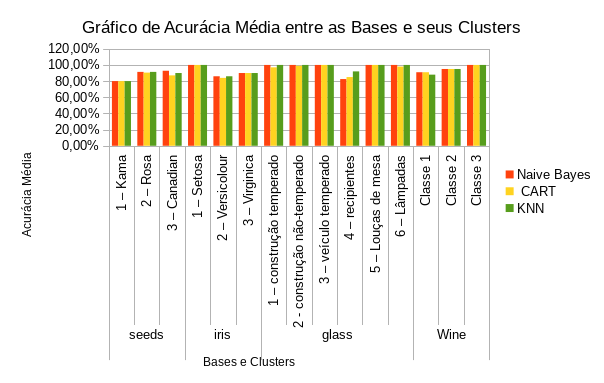
\includegraphics[scale=0.9]{figs/grafico_acuracia_media_algoritmos.png}
        \caption{Acurácia Média dos Rótulos dos Algoritmos: Naive Bayes, CART e KNN} \label{fig:acuracia_media_algoritmos}
\end{figure}

Uma breve análise do gráfico da figura \ref{fig:acuracia_media_algoritmos} referente as acurácias dos rótulos, fica claro que a qualidade deles foram satisfatórias, pois atingiram uma acurácia média com mínimo de 80\%. A acurácia desses rótulos servem para mostrar o quanto esses rótulos representam o grupo através das amostras testadas, e os três algoritmos tiveram acurácias bem parecidas, e em específico o Naive Bayes e KNN. Os clusters com menores acurácias 

Uma forma de comprovar a qualidade do rótulo e mostrar que de fato ele cumpre seu papel de identificar o grupo, é colocar em prática um exemplo que pode ser visto na figura \ref{fig:grafico_iris_petalwidth_petallength_BrOf}. Para essa análise foi selecionada a base Iris, por possuir poucos atributos e também pelos rótulos encontrados em todos os \textit{clusters} variarem entre dois deles: petalwidth e petallength. 

%Dessa forma o gráfico da figura \ref{fig:grafico_iris_petalwidth_petallength_BrOf} apresenta o comportamento dos dados desta base, logo facilita a análise para comfirmar se os rótulos encontrados cumprem a finalidde de representar os grupos. 

O gráfico da figura \ref{fig:grafico_iris_petalwidth_petallength_BrOf} exibe a relação de dois atributos representados pelos eixos X e Y, facilitando a visualização do comportamento dos três grupos: \textit{Iris-setosa}, \textit{Iris-versicolor} e \textit{Iris-viginica}.

\begin{figure}[h!]
        \centering
        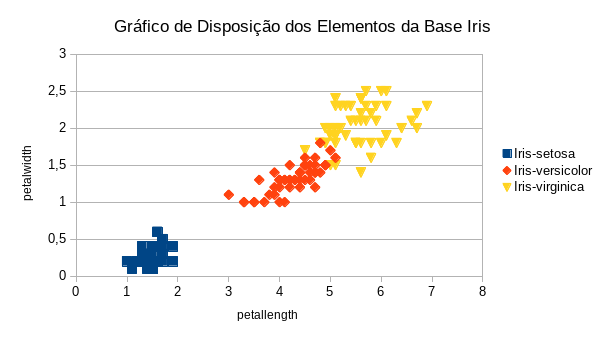
\includegraphics[scale=0.9]{figs/grafico_iris_petalwidth_petallength_BrOf.png}
        \caption{Gráfico da disposição de elementos da Base Iris entre os eixos \textbf{petallength} e \textbf{petalwidth}} \label{fig:grafico_iris_petalwidth_petallength_BrOf}
\end{figure}

De acordo com a proposta dessa pesquisa, sobre a rotulação de dados, e para mostrar a confiabilidade dos rótulos encontrados nas bases de dados na representação dos clusters, foi inserido como exemplo a base Iris representada acima através da figura \ref{fig:grafico_iris_petalwidth_petallength_BrOf}, para uma análise dos rótulos. Todos os algoritmos: Naive Bayes, CART e KNN, encontraram os mesmos rótulos no \textit{cluster} 1 da Iris, e ao analisar o gráfico, o \textit{cluster} 1 (Iris-setosa), é possível perceber uma relação bem definida entre os demais grupos, pois de fato, todos os elementos que possuem comprimento da pétala (\textit{petallength}) variando de 1.0 até 3.7 e largura de pétala (\textit{petallength}) variando de 0.1 a 1.0 participa do grupo Iris-setosa, portanto, esse rótulo comprovadamente representa este grupo.

Analisando os outros grupos através do gráfico da figura \ref{fig:grafico_iris_petalwidth_petallength_BrOf} percebe-se que a amostra de dados dos grupos Iris-versicolor e Iris-virginica contêm elementos que se misturam, não deixando um ponto de corte tão preciso quanto o da Iris-setosa, ocasionando ao rótulo alguns erros identificados nos \textit{clusters} 1 e 2.
